\documentclass[11pt,twoside]{report} %please use 11pt for your report

\usepackage[english]{babel}
\usepackage[utf8]{inputenc}
\usepackage[T1]{fontenc}

\usepackage[a4paper,top=2.5cm,bottom=2.5cm,width=15cm]{geometry}

\usepackage{afterpage}

%%%% MY STUFF %%%%
% exponential e
\newcommand{\me}{\mathrm{e}}
% imaginary i
\newcommand{\mi}{\mathrm{i}}
% differential operator
\newcommand{\md}{\mathrm{d}}
% bracketed matrix
\newcommand{\bmat}[1]{\begin{bmatrix}#1\end{bmatrix}}
% fast epsilon
\newcommand{\eps}{\epsilon}
% bracketed equation
%\newcommand{\equation}[1]{\begin{equation}#1\end{equation}}
% bracketed align
%\newcommand{\align}[1]{\begin{align}#1\end{align}}


% bold fonts in math mode
%\usepackage{bm}

\usepackage{physics}
\usepackage{tikz-feynman}
\usepackage{wrapfig}
\usepackage{subcaption}
\usepackage{siunitx}

% why is this not defined in the package
\DeclareSIUnit\year{year}
\DeclareSIUnit\kt{\kilo\tonne}

\captionsetup{font=small}

%%%%%%%%%%%%%%%%


\newcommand\blankpage{%
    \null
    \thispagestyle{empty}%
    \addtocounter{page}{-1}%
    \newpage}

\usepackage{graphicx}
\graphicspath{ {./images/} }

%\usepackage{babel,csquotes,xpatch}
%\usepackage[backend=biber,style=authoryear]{biblatex}
%\addbibresource{ref.bib}

%% Useful packages
%%Mathematical typesetting https://michael-prokop.at/latextug/amsldoc.pdf
\usepackage{amsmath}
\usepackage{caption}
%%Adds to do notes and lists http://tug.ctan.org/macros/latex/contrib/todonotes/todonotes.pdf
\usepackage[colorinlistoftodos]{todonotes}
%%Uncomment below for internal hyperlinks
\usepackage{hyperref}
\usepackage{xcolor}
\definecolor{nh}{RGB}{50, 142, 237}

\hypersetup{
	colorlinks = true,
	allcolors = nh,
}
%Floating figures and tables
\usepackage{float}
%%Drawing Package
%%\usepackage{pgf,tikz}\usepackage{mathrsfs}\usetikzlibrary{arrows}\pagestyle{empty}
%%\usepackage{tikzscale}
%% Clipping and trimming images http://mirrors.ibiblio.org/CTAN/macros/latex/contrib/adjustbox/adjustbox.pdf
\usepackage[export]{adjustbox}

\begin{document}
\begin{titlepage}
\begin{center}

\vspace*{4cm} % adjust as you wish
        
	{\Large\textbf{Experimental sensitivity of future neutrino oscillation experiments}}
        
\vspace{1cm} % adjust as you wish
      

{\large Candidate Number: 133856

Supervisor: Dr. Elisabeth Falk\\

Word Count: 9283\\

	Date: 18 May 2018\\
        
}

\vspace{8cm} % adjust as you wish

\includegraphics[width=100px]{sussexLogo}\\

{\Large\textbf{University of Sussex}}
\end{center}
\end{titlepage}


\begin{center}

\vspace*{2cm} % adjust as you wish
        
{\large\textbf{Abstract}}
        
\vspace{1cm} % adjust as you wish
\end{center}


{\bf Your abstract should be at least as long as the first paragraph in this example.} Lorem ipsum dolor sit amet, consectetur adipiscing elit. Nulla tincidunt bibendum lacus ac finibus. Nam ornare justo ipsum, sit amet placerat arcu sodales non. Curabitur posuere tortor vel magna venenatis, vitae mattis lectus eleifend. Nunc imperdiet eros aliquam nunc imperdiet, ac semper dui porttitor. Nulla pretium, ante id feugiat finibus, urna lectus ultrices nulla, quis placerat libero nibh eget justo. Vestibulum nec felis sed eros tempus elementum. Praesent urna nulla, volutpat eu quam dignissim, maximus tincidunt sapien. Nulla facilisi. Praesent diam est, suscipit et risus eget, dapibus egestas lectus. Maecenas interdum ante ut tortor tempor, eu sodales elit lobortis.
Lorem ipsum dolor sit amet, consectetur adipiscing elit. Nulla tincidunt bibendum lacus ac finibus. Nam ornare justo ipsum, sit amet placerat arcu sodales non. Curabitur posuere tortor vel magna venenatis, vitae mattis lectus eleifend. Nunc imperdiet eros aliquam nunc imperdiet, ac semper dui porttitor. 

{\bf It is fine to use paragraph breaks in an abstract.} Lorem ipsum dolor sit amet, consectetur adipiscing elit. Nulla tincidunt bibendum lacus ac finibus. Nam ornare justo ipsum, sit amet placerat arcu sodales non. Curabitur posuere tortor vel magna venenatis, vitae mattis lectus eleifend. Nunc imperdiet eros aliquam nunc imperdiet, ac semper dui porttitor. Nulla pretium, ante id feugiat finibus, urna lectus ultrices nulla, quis placerat libero nibh eget justo. Vestibulum nec felis sed eros tempus elementum. 
Lorem ipsum dolor sit amet, consectetur adipiscing elit. Nulla tincidunt bibendum lacus ac finibus. Nam ornare justo ipsum, sit amet placerat arcu sodales non. Curabitur posuere tortor vel magna venenatis, vitae mattis lectus eleifend. Nunc imperdiet eros aliquam nunc imperdiet, ac semper dui porttitor. Nulla pretium, ante id feugiat finibus, urna lectus ultrices nulla, quis placerat libero nibh eget justo. Vestibulum nec felis sed eros tempus elementum. Praesent urna nulla, volutpat eu quam dignissim, maximus tincidunt sapien. Nulla facilisi. Praesent diam est, suscipit et risus eget, dapibus egestas lectus. Maecenas interdum ante ut tortor tempor, eu sodales elit lobortis. {\bf Your abstract should fit onto a single page.}

\tableofcontents % required
%\listoftables % optional
%\listoffigures % optional

\thispagestyle{empty}

\clearpage
\pagenumbering{arabic}

\chapter*{Preface}
\addcontentsline{toc}{chapter}{Preface}
%\begin{center}
%
%\vspace*{2cm} % adjust as you wish
%        
%{\large\textbf{Preface}}
%        
%\vspace{1cm} % adjust as you wish
%\end{center}

This dissertation is a report of the work that was done from September 2017 to
April 2018, as part of an MPhys final year project.

Where mathematical derivations are presented that are not a product of our
original work, we make it known explicitly and provide a reference to the
original author(s).


All graphs shown in this report are results of our neutrino oscillation
model, with the exception of figure~\ref{fig:nuflux} which is a reproduction
from the DUNE Conceptual Design Report\cite{cdr}. The ROOT framework\cite{ROOT}
is used to produce the plots.
The model is a C++ implementation of the formalism of chapter~\ref{ch:osc} and
the statistics of section~\ref{sec:statistics}. For
reference, it is available publicly at
\href{url}{https://github.com/beulard/nuosc}.
In order to evaluate experimental sensitivities, the code requires predicted
integrated event rates to be provided as inputs. In the case of DUNE and Hyper-K,
these are estimated from performance estimates of the beamline and detector,
and are presented in their respective design reports\cite{cdr, hyperk}.

Our results are unique but not original, as similar results can be found ---
and are often referenced throughout the text --- in the neutrino oscillation
physics literature.


%You do not get extra marks from including a preface, but you will have marks
%deducted if you do not! The purpose of the “preface” is for you to state
%explicitly the extent to which your dissertation relies on the work of others,
%and highlight the portion that you claim to be your own original work.  Without
%this statement, it will be assumed that none of the work is your own, and that
%your report is simply a review of what other people have done. Please discuss
%with your supervisor to ascertain what, if any, of the work you have done is
%not just new to you, but new to the field, i.e. original research. If there are
%any aspects of your project are original, however small, and even if achieved
%in collaboration with others, make sure this is made very clear in the preface
%and abstract. 
%b.	An example preface is as follows: “Chapter 1 is review material (all
%references are given in Section 7). The data in section 2.1 were provided by my
%supervisor.  The analysis in section 3.2 was carried out using codes that were
%adapted from those developed by PhD Student Santa Claus. I wrote the codes used
%to carry out the analysis in Chapter 4 from scratch. The results presented in
%5.1 are, the best of the knowledge of my supervisor and I, original and are
%currently being prepared for publication in a refereed journal. The derivation
%included in Appendix B was carried out by myself before the final year project
%time period.” 


\chapter{Introduction}
% This chapter gives reader the background knowledge they will need in order to understand the following chapters. This should not include descriptions of the work you have done, but it should provide the motivation for why you did it.  Some reports will have two chapters of background material (e.g. one on general background from books, and one providing a review of journal articles you have read).
\label{ch:introduction}
This dissertation is a report of the steps that were taken in order to predict the
sensitivity of a future neutrino experiment to the neutrino mass hierarchy and
to CP violation.
The work that was done heavily relies on the quantum mechanical description of
neutrino oscillations and the implementation thereof in a self-contained C++
framework.

For this reason, we start chapter~\ref{ch:osc} by introducing the neutrino and the
concept of neutrino oscillations with its associated formalism. From the
starting point that neutrino flavour eigenstates are different from neutrino
mass eigenstates, we derive the probability of a neutrino changing flavour
after travelling through empty space. 

In our model of a neutrino experiment, we use the assumption that three
neutrino flavours exist and that a neutrino produced in a particular flavour
can oscillate to the other two and back. Hence we introduce the mixing matrix
for three flavours, known as the PMNS matrix, and discuss the presence in this
matrix of the imaginary phase $\me^{\mi\delta_{CP}}$ which could be responsible for CP
violation in the lepton sector.

Because the neutrino experiments under consideration are long-baseline
underground experiments, it is necessary to treat the flavour oscillations not
in vacuum but in matter. We show a derivation of the corrections that must be
applied in the case where only two neutrinos oscillate and discuss how one can
extend to the three neutrino case.

In order to provide motivation for our work, we discuss the current state of
neutrino oscillations, namely which parameters are known and which parameters
require higher precision experiments in order to be measured.


While chapter~\ref{ch:osc} covers the fundamental principles at work, some elements of
statistics also need to be discussed. Evaluating the sensitivity of an
experiment requires the formal definition of a relevant test statistic, which
then has to be evaluated from our model of the experiment. In order to make the
results meaningful, we must also discuss the interpretation of such a test
statistic in the context of an experiment which has yet to be performed.
The statistics are discussed in the first part of chapter~\ref{ch:methods}.

We then present the oscillation probabilities resulting from our
implementation of the formalism of chapter~\ref{ch:osc} and try to outline some
relevant features. 

The whole purpose of such a model is to apply it to a real neutrino experiment
and study the potential outcomes and discoveries that it could bring.
We chose the Deep Underground Neutrino Experiment (DUNE) as our main
application. Because it is already a very mature project, a multitude of
extremely detailed resources are available, such as the four-volume conceptual
design report\cite{cdr-all} (CDR). Using information and results from the CDR
lets us cirumvent the in-depth modelling of a neutrino beam and detector, and
focus on the oscillations instead. This is discussed in detail in the second
half of chapter~\ref{ch:methods}.

Finally, we combine all the information of chapter~\ref{ch:methods} into our
predictions of the sensitivity of DUNE to CP violation and to the neutrino mass
hierarchy.
As a short extra example, we produce similar results for the shorter-baseline
Hyper-Kamiokande (Hyper-K) experiment and use that as a reference to
compare to DUNE.


%This chapter introduces the report and tells the reader what they should expect
%to see in the next chapters. We should introduce the contents of the
%following two chapters in a qualitative way and maybe give some context and
%motivation for the research.


\chapter{Neutrinos and oscillations}
\label{ch:osc}
We will now give an overview of the theoretical concepts that are used
throughout this report. We will present a review of neutrino flavour
oscillations in a vacuum, for the commonly considered cases of two and three
neutrino flavours. We will derive the oscillation probability for
neutrinos in matter with a constant density, in the simpler case of two
neutrinos. In the last section, the current state of neutrino oscillations will
be reviewed in order to provide motivation for the following chapter.


\section{History of the neutrino}
The neutrino particle was first postulated by Wolfgang Pauli in 1930 to explain
the continuous energy distribution of the electron in beta decays, in his
famous letter to the Physics Institute of Zürich\cite{pauli}. 

Its existence was confirmed in 1956 by Cowan and Reines\cite{cowan} through the
observation of anti-neutrinos from a nuclear reactor being captured by protons
in a water tank.
A number of subsequent experiments were designed to map out the properties of
the neutrino and its interactions\cite{zuber}. As of today, the neutrino is
still not fully understood, and neutrino physics has become one of the leading
branches of experimental particle physics along with collider physics. 

The existence of distinct flavours of neutrinos was first investigated by
Bruno Pontecorvo\cite{pontecorvo} in 1959. He proposed that a weak interaction
involving charged leptons ($e$, $\mu$) discriminates between neutrino flavours,
hence a process such as $\nu_\mu + n \rightarrow e^- + p$ is forbidden.
This was confirmed in 1962 by Danby et al.\cite{danby} at the Brookhaven
National Laboratory, where they showed that electron-neutrinos and
muon-neutrinos were in fact distinct particles.
This was also a first hint at the possibility of neutrino flavour oscillations,
which Pontecorvo\cite{pontecorvo-osc} started theorizing in 1967.
In 2000, the DONUT experiment\cite{donut} reported the observation of
tau-neutrino interactions, hence further corroborating the theory of the
three neutrino flavours.

As will be discussed later, the fact that a neutrino can change its flavour by
propagating through empty space is direct evidence that neutrinos are massive
particles, unlike what is initially described by the Standard Model.
The 2015 Nobel Prize was awarded to the Super-K and Sudbury Neutrino
Observatory (SNO) collaborations for the discovery of neutrino oscillations in
1999 and 2001\footnote{In fact, SNO observed oscillations in matter, known as
the MSW effect\cite{smirnov}, while Super-K observed oscillations in
vacuum.}, respectively.

Although neutrino oscillations have been observed, some of the physical parameters that
govern this process remain difficult to probe because of the elusiveness of
neutrinos: being only involved in weak processes, they require extremely
voluminous detectors in order to get the slightest signal.
The Deep Underground Neutrino Experiment (DUNE) in the United States and the
upgrade to Super-Kamiokande, Hyper-Kamiokande in Japan, are examples of
future experiments that aim to determine these parameters.

In the Standard Model, there are twelve elementary fermions: six quarks and six
leptons (plus their respective antiparticles). The leptons consist of three
charged leptons $(e, \mu, \tau)$ and three corresponding charge-less neutrinos
$(\nu_e, \nu_\mu, \nu_\tau)$. The electron neutrino $\nu_e$, for example, is
the neutrino which can interact weakly with an electron and a
$W$ boson~(Fig.~\ref{fig:weak_vertex}). 

\begin{wrapfigure}{r}[1.5cm]{0.2\textwidth}
	\includegraphics{images/weak_vertex.pdf}
	\captionsetup{justification=centering}
	\caption{The weak vertex for an electron neutrino.}
	\label{fig:weak_vertex}
\end{wrapfigure}

Neutrinos, being leptons (colorless) and carrying zero charge, interact only via the weak
interaction, which makes them impossible to observe directly. Their existence
and their properties can only be inferred from their interactions with other
particles.
Experimentally, only left-handed neutrinos and right-handed
anti-neutrinos are observed. In the Standard Model, this curious property
prevents the neutrinos from acquiring a mass through interactions with the
Higgs field in the same way that charged leptons do\cite{schwichtenberg}. Hence
the Standard Model on its own cannot accurately describe neutrinos, and
extensions such as the seesaw mechanism or extra dimensions are needed. This
discussion lies beyond the scope of this report since we are only concerned
with the phenomenological description of neutrino oscillations, which is
achieved via straightforward quantum mechanics in the next section.

\section{Neutrino oscillations}
We will now introduce the mathematical tools that we use to describe neutrino
oscillations. 

It is now known experimentally that 
the neutrino flavours ($\nu_e, \nu_\mu, \nu_\tau$) mix when propagating through
space\cite{superk}. This process is structurally similar to the quark generation
mixing between down, strange and bottom quarks\cite{pdg_ckm}
and is direct evidence that for neutrinos and quarks, the weak
eigenstates\footnote{Weak eigenstate: state which interacts with the W, Z
bosons.} are not in one-to-one correspondence with the mass
eigenstates\footnote{Mass eigenstate: state which has definite mass and
propagates through space as a wave.}.

In the Standard Model, the W bosons mediate the interactions between up-type and
down-type quarks, and between charged leptons and neutrinos. 
When describing these particles, it is useful to express them either in the
weak eigenbasis for interactions or in the mass eigenbasis for
free-propagation.
For down-type quarks and neutrinos, these bases are not identical: their
relationship is conventionally represented by the Cabibbo-Kobayashi-Maskawa
(CKM) matrix and the Pontecorvo-Maki-Nakagawa-Sakata (PMNS) matrix,
respectively.  This allows down-type quarks to interact with up-type quarks of
a different generation, or, as we shall see, it allows neutrinos to change their
flavour composition as they propagate in empty space.


\subsection{Neutrino oscillation formalism} 
The following derivations are heavily inspired by chapter 8 of~\cite{zuber}.
Let us consider a general system where there exist $n$ neutrino flavours. 
We mentioned the two eigenbases of interest: the weak (flavour)
eigenstates $\ket{\nu_{\alpha}}$ where $\alpha$ is a lepton flavour,
$\alpha=l_1, l_2, ..., l_n$, and the mass eigenstates $\ket{\nu_i}$, $i=1, 2,
..., n$. 
Flavour eigenstates interact with matter through the weak interaction, and
hence are the states we observe in nature. Eigenstates are orthogonal within
each basis:
$$
\bra{\nu_\alpha}\ket{\nu_\beta} = \delta_{\alpha \beta}, \quad
	\bra{\nu_i}\ket{\nu_j} = \delta_{ij}  \quad
$$
and the two bases are related by a $n\times n$ unitary matrix $U$:
\begin{align}
	&\ket{\nu_\alpha} = \sum_i U_{\alpha i} \ket{\nu_i}\label{eq:bases1}\\
	&\ket{\nu_i} = \sum_\gamma (U^\dagger)_{i \gamma} \ket{\nu_\gamma} = \sum_\gamma
			U^*_{\gamma i} \ket{\nu_\gamma}\label{eq:bases2}\\
	&U^\dagger U = 1, \nonumber
\end{align}
where greek letters denote indices in the flavour basis and latin letters
denote indices in the mass basis.

The mass eigenstates are solutions of the free Hamiltonian in a vacuum, hence
they are stationary states and evolve in time as $\ket{\nu_i(x,
t)} = \me^{-\mi E_i t} \ket{\nu_i(x, 0)}$, where $\ket{\nu_i(x, 0)} = \me^{\mi p
x} \ket{\nu_i}$ for a plane wave neutrino produced at $x=0$.
Hence a neutrino produced as a flavour eigenstate $\alpha$ would have the
following time dependence:
\begin{align*}
\ket{\nu_\alpha(x, t)} &= \sum_i U_{\alpha i} \ket{\nu_i(x, t)} \\
		&= \sum_i U_{\alpha i} \me^{-\mi E_i t} \me^{\mi p x} \ket{\nu_i}\\
		&= \sum_{i, \gamma} U_{\alpha i} U^*_{\gamma i} \me^{\mi p x}
				\me^{-\mi E_i t} \ket{\nu_\gamma}\quad\text{(using eq.~\ref{eq:bases2})}.
\end{align*}
Note that we are working in natural units where $c=\hbar=1$ for clarity. When
implementing this formalism in code, the units must be restored using
the usual conversion factors in order to get accurate numerical results.
The transition amplitude to a flavour $\beta$ is thus 
\begin{align}
	A_{\alpha \rightarrow \beta}(x, t) = \bra{\nu_\beta}\ket{\nu_\alpha(x, t)} \nonumber
			= \sum_i U^*_{\beta i} U_{\alpha i} \me^{\mi p x}
			\me^{-\mi E_i t}\quad\text{(using eq.~\ref{eq:bases1})}.
\end{align}
By assuming that all neutrinos have small masses, and thus are highly
relativistic, we are able to perform a binomial approximation on their
energy: 
\begin{equation} E_i = \sqrt{m_i^2 + p^2} \simeq p + \frac{m_i^2}{2 p} \simeq E +
\frac{m_i^2}{2E},\label{eq:binomial}\end{equation}
where we call $E \approx p$ the neutrino energy at the source\footnote{As
pointed out by Cohen, Glashow and Ligeti\cite{cohen}, we are taking a shortcut
here by assuming that the weak eigenstate comes out as a linear superposition
of mass eigenstates with equal energies. However our description leads to
identical oscillation formulae as a more physically rigorous one where particle
entanglement after the interaction is taken into account. We choose to keep
this derivation and skip the details for the sake of simplicity.}. We call $L$
the distance from the neutrino source to the detector, known as the baseline.
Under our relativistic assumption, we have $L \approx t$. Going back to the
transition amplitude,
\begin{align*}
	A_{\alpha \rightarrow \beta}(L, E) &= \sum_i U^*_{\beta i} U_{\alpha i}
	\exp(\mi E L - \mi(E + \frac{m_i^2}{2 E}) L)\\
	&= \sum_i U^*_{\beta i} U_{\alpha i} \exp(-\mi \frac{m_i^2 L}{2E}),
\end{align*}
The transition probability is then
\begin{align}
	\label{eq:nuprob}
	P_{\alpha \rightarrow \beta}(L, E) &= |A_{\alpha \rightarrow \beta}(L, E)|^2 \nonumber\\
	&= \sum_i \sum_j U_{\alpha i} U^*_{\beta i} U^*_{\alpha j} U_{\beta j}
	\exp(-\mi \frac{\Delta m_{ij}^2}{2} \frac{L}{E}),
\end{align}
where $\Delta m^2_{ij} = m^2_i - m^2_j$ is the mass squared difference between
two mass eigenstates.
The analysis is similar when considering anti-neutrinos except that $U$ must be
replaced by $U^*$ everywhere and vice-versa.

The formula we have derived here is the general probability of oscillation from a
flavour eigenstate $\ket{\nu_\alpha}$ to another flavour eigenstate
$\ket{\nu_\beta}$. This effectively describes the probability that after
travelling a distance $L$, the neutrino wavefunction will collapse into a
$\beta$ flavoured neutrino if it interacts in our detector.
In the following sections, we apply this formalism to two-neutrino and
three-neutrino systems. 



\subsection{Two-neutrino oscillations}\label{sec:twonu}
The case for two neutrino eigenstates is the simplest to consider. The
unitary nature of the mixing matrix $U$ and the arbitrarity of the complex phases
of quantum states reduces the number of observable mixing parameters to
one\cite{langacker}.
An enlightening way to write the mixing matrix is\cite{zuber} 
\begin{equation}
	\begin{bmatrix} \nu_\mu \\ \nu_\tau \end{bmatrix} =
	\begin{bmatrix} \cos\theta & \sin\theta \\
								 -\sin\theta & \cos\theta \end{bmatrix}
	\begin{bmatrix} \nu_1 \\ \nu_2 \end{bmatrix},
		\label{eq:twonumixing}
\end{equation}
where $\theta$ is called the mixing angle.
We see here that the two eigenbases are analogous to two sets of Cartesian axes
in two dimensions, one being rotated by an angle $\theta$ with respect to the
other.

We use the $\mu$ and $\tau$ flavours here in reference to the
atmospheric neutrino experiment at Super-Kamiokande\cite{superk} (Super-K): for
neutrinos produced by cosmic rays in the atmosphere, it is a good approximation
to consider a two-neutrino oscillation between the $\mu$ and $\tau$ flavours,
and to neglect the $\nu_\mu \rightarrow \nu_e$ channel. 
This simple mixing matrix can be substituted in eq.~\ref{eq:nuprob} to obtain a
more concrete oscillation probability:
\begin{align}
	P_{\nu_\mu \rightarrow \nu_\tau}(L, E) &= U_{\mu 1}^2 U_{\tau 1}^2 + U_{\mu 2}^2
	U_{\tau 2}^2 \nonumber\\&\quad+ U_{\mu 1} U_{\tau 1} U_{\mu 2} U_{\tau 2} \bigg[\exp(-\mi
	\frac{\Delta m_{12}^2 L}{2 E}) + \exp(-\mi \frac{\Delta m_{21}^2 L}{2
	E})\bigg]\nonumber\\
	&= \cos^2\theta \sin^2\theta\enskip \bigg[2 - 2\cos\frac{\Delta m_{21}^2 L}{2
	E}\bigg]\nonumber\\
	&= \sin^2(2\theta)\sin^2\bigg(\frac{\Delta m^2}{4}
	\frac{L}{E}\bigg),\label{eq:twonu}
\end{align}
where in the first step we have used the fact that $\Delta m_{12}^2 = m_1^2 -
m_2^2=-(m_2^2 - m_1^2) = -\Delta m_{21}^2$ to bring the exponentials into
cosine form.
Note that there are only two mass eigenstates here, hence we define $\Delta m^2
\equiv \Delta m_{21}^2$.

This example is particularly informative, as one can clearly see the role of
each parameter in the oscillation probability. The first term is a constant
which depends on the mixing angle, and must be determined by experiment. For
$\theta = \frac{\pi}{4}$, the mixing is maximal and the probability is allowed
to increase up to 100\%. The second term is manifestly oscillatory. Its
frequency is determined by the mass difference $\Delta m^2$, which may also be
determined by fitting experimental data. Note also that if the mass squared
difference is zero, the oscillation probability is zero. This implies that
oscillations are only possible if at least one of the mass eigenstates has a
non-zero mass.
Evidently, since there are only two flavours, the probability of $\nu_\mu$
``survival'' is
$$P_{\nu_\mu \rightarrow \nu_\mu}(L, E) = 1 - P_{\nu_\mu \rightarrow
\nu_\tau}(L, E).$$



\subsection{Three neutrino oscillations}
When we consider three eigenstates, the number of parameters is increased to
four\cite{langacker}:
three mixing angles $\theta_{12}, \theta_{13}$ and $\theta_{23}$, and an
imaginary phase $\delta_{CP}$. This so called CP-violating phase gives rise to
a difference between oscillation probabilities of neutrinos and anti-neutrinos,
hence it allows violation of the charge-parity (CP) symmetry. 
The mixing matrix can be written in a suggestive way as
\begin{equation}\label{eq:PMNS}
U_{\mathrm{PMNS}} = 
\begin{bmatrix} 1 & 0 & 0 \\ 0 & c_{23} & s_{23} \\ 0 & -s_{23} & c_{23} \end{bmatrix}
\begin{bmatrix} c_{13} & 0 & s_{13} \me^{-\mi \delta_{CP}} \\ 0 & 1 & 0 \\
								-s_{13} \me^{\mi \delta_{CP}} & 0 & c_{13} \end{bmatrix} 
\begin{bmatrix} c_{12} & s_{12} & 0 \\ -s_{12} & c_{12} & 0 \\ 0 & 0 & 1 \end{bmatrix}
,\end{equation}
where $c_{ij} = \cos(\theta_{ij})$ and $s_{ij} = \sin(\theta_{ij})$.
This form is analogous to a 3D rotation around three Euler angles, except for
the appearance of $\delta_{CP}$ in the ``13'' rotation.

Unlike in the two-neutrino case, substituting this mixing matrix into
eq.~\ref{eq:nuprob} turns out not to be very insightful. It is important
however to underline all the oscillation parameters that are present here.
Along with the four mixing parameters in the PMNS matrix, we have three mass
squared differences $\Delta m^2_{31},~\Delta m^2_{32}$ and $\Delta m^2_{21}$,
of which two are independent since $\Delta m^2_{32} + \Delta m^2_{21} = \Delta
m^2_{31}$. This leaves six independent
parameters that must be determined by oscillation experiments.
In section~\ref{sec:state}, we will go over the current state of our knowledge
of these parameters, which will provide motivation for the work presented in
chapter~\ref{ch:methods}.


\subsection{Neutrino oscillations in matter}
So far we have only discussed neutrino oscillations in vacuum, where no weak
interactions take place.
In matter, where atoms are present, neutrinos can undergo coherent forward
scattering off of atomic electrons, modifying the oscillation probability over
large enough distances. This is known as the Mikheyev-Smirnov-Wolfenstein (MSW)
effect\cite{wolfenstein, mikheyev-smirnov}, or simply matter effect.
\begin{figure}
	\centering
	\begin{subfigure}{0.3\textwidth}
		\centering
	\feynmandiagram[small, vertical=a to b]{
		ni [particle=\(\nu_e\)] -- [fermion] b -- [fermion] ef [particle=\(e^-\)],
		a -- [boson, edge label=\(W\)] b,
		ei [particle=\(e^-\)] -- [fermion] a -- [fermion] nf [particle=\(\nu_e\)],
		};
		\caption{Electron-neutrino scattering.}
		\label{fig:nu_e-scatter}
	\end{subfigure}
	\begin{subfigure}{0.3\textwidth}
		\centering
		\feynmandiagram[small, horizontal=a to b]{
			ei [particle=\(e^-\)] -- [fermion] a -- [fermion] ni
			[particle=\(\bar{\nu}_e\)],
			a -- [boson, edge label=\(W^-\)] b,
			nf [particle=\(\bar{\nu}_e\)] -- [fermion] b -- [fermion] ef
			[particle=\(e^-\)],
			};
			\caption{Anti-$\nu_e$ scattering.}
			\label{fig:anti-nu_e-scatter}
	\end{subfigure}
	\begin{subfigure}{0.3\textwidth}
		\centering
		\feynmandiagram[small, vertical=a to b]{
			ni [particle=\(\nu_{e,\mu,\tau}\)] -- [fermion] b -- [fermion] nf
			[particle=\(\nu_{e,\mu,\tau}\)],
			a -- [boson, edge label=\(Z\)] b,
			ei [particle=\(e^-\)] -- [fermion] a -- [fermion] ef [particle=\(e^-\)],
		};
		\caption{Scattering through $Z$ boson affects all flavours equally.}
		\label{fig:z-scatter}
	\end{subfigure}
	\caption{The three possible tree-level interactions of neutrinos with atomic
	electrons in matter.}
\label{fig:forward_scatter}
\end{figure}

A neutrino can scatter either by exchanging a $W^\pm$ boson --- known as
charged current (CC) interaction --- or by exchanging a $Z$ boson --- neutral
current (NC) interaction. The neutral current interaction is experienced
equally by all three flavours (fig.~\ref{fig:z-scatter}), hence it does not
have an effect on the relative
propagation phases, and causes no change in the oscillation probability. The
charged current is specific to the neutrino flavour. Since only
electrons are present in matter, only electron neutrinos are subject to CC
interactions~(figs.~\ref{fig:nu_e-scatter},~\ref{fig:anti-nu_e-scatter}). 
Hence electron neutrinos propagating in matter pick up a different phase than
if they were propagating in empty space. This can be implemented in the
oscillation formalism by adding a potential term to the Hamiltonian for
electron neutrinos only. This term will be proportional to the density of
matter and to the weak coupling constant\cite{zuber}.

In what follows, we derive the corrections that must be applied to the
oscillation formalism for two neutrino flavours, in order to accurately
describe oscillations in matter.
This derivation is inspired by section~8.9 of Kai Zuber's textbook\cite{zuber}
and Stefania Ricciardi's notes on oscillations in matter\cite{ricciardi}.

We start from the time evolution of two mass eigenstates (Schrödinger's
equation):
\begin{align}
	\mi \frac{\md}{\md t} \begin{bmatrix} \nu_1 \\ \nu_2 \end{bmatrix}
		&= \hat{H}_\text{mass} \begin{bmatrix} \nu_1 \\ \nu_2
		\end{bmatrix}\nonumber \\
		&= \begin{bmatrix} E_1 & 0 \\ 0 & E_2 \end{bmatrix} \begin{bmatrix} \nu_1
\\ \nu_2 \end{bmatrix}\nonumber \\
&= \frac{1}{2E} \bmat{m^2_1 & 0 \\ 0 & m^2_2} \bmat{\nu_1 \\ \nu_2} + \bmat{E &
0 \\ 0 & E} \bmat{\nu_1 \\ \nu_2},\label{eq:massvacuum}
\end{align}
where in the last step we used the approximation of eq.~\ref{eq:binomial}.
The second term is a multiple of the identity, and only contributes a common phase to
the wavefunctions $\nu_1$ and $\nu_2$. It does not affect the oscillations, and
will be discarded in what follows.
Now we transform into the flavour basis by using $\ket{\nu_\text{mass}} =
U^\dagger \ket{\nu_\text{flavour}}$ (eq.~\ref{eq:bases2}), and multiply by $U$ on the left:
\begin{align*}
	\mi \frac{\md}{\md t}\bigg( U^\dagger \bmat{ \nu_e \\ \nu_\mu
	}\bigg)
		&= \frac{1}{2E}\bmat{m^2_1 & 0 \\ 0 & m^2_2} U^\dagger \bmat{\nu_e
			\\ \nu_\mu} \\
		\implies 
	\mi \underbrace{U U^\dagger}_{=1} \frac{\md}{\md t}\bmat{\nu_e \\ \nu_\mu}
		&= \underbrace{\frac{1}{2E} U \bmat{m^2_1 & 0 \\ 0 & m^2_2}
			U^\dagger }_{\equiv \hat{H}_{\text{flavour}}} \bmat{\nu_e
			\\ \nu_\mu}.
\end{align*}
For this illustration, our two flavours are $\nu_e$ and $\nu_\mu$ because matter effects play
an important role in the oscillations between those two, for example
in long baseline experiments, or for solar neutrinos.
We use the explicit form of $U$ for two neutrinos (eq.~\ref{eq:twonumixing}) to
determine $\hat{H}_\text{flavour}$. The result is
\begin{equation}\hat{H}_\text{flavour} = \frac{\Delta m^2}{4 E} \bmat{-\cos 2\theta & \sin
	2\theta \\ \sin 2\theta & \cos
2\theta},\label{eq:flavourvacuum}\end{equation}
where $\Delta m^2 = m_2^2 - m_1^2$, and we have subtracted a multiple of the
identity. Our goal, after introducing the extra potential in matter, will be to
express the flavour Hamiltonian in this form, albeit with different $\Delta
m^2$ and $\theta$, and to relate it to the mass eigenstates in matter. This
will ensure that we can simply apply the steps of section~\ref{sec:twonu} and
directly obtain the oscillation formula.

In matter, the electron neutrinos interact with electrons, so we must add a
potential term $V_e$ to the Hamiltonian. For simplicity, we assume that this
term is constant, i.e. that the density of matter is constant. This assumption
is fairly accurate for neutrinos propagating in the Earth's crust, but not for
solar neutrinos, for example. The Hamiltonian in matter is
\begin{equation}
	\hat{H}^m_\text{flavour} = \frac{\Delta m^2}{4 E} \bmat{-\cos 2\theta & \sin
	2\theta \\ \sin 2\theta & \cos 2\theta} + \bmat{V_e & 0 \\ 0 &
	0}.\label{eq:matter_potential}
\end{equation}
Again, we subtract a multiple of the identity $V_e / 2$ without affecting the
oscillations:
\begin{equation}\hat{H}^m_\text{flavour} = \frac{\Delta m^2}{4 E} \bmat{-\cos 2\theta + A & \sin
2\theta \\ \sin 2\theta & \cos 2\theta - A},\label{eq:flavourmatter1}\end{equation}
where $A = 2 E V_e / \Delta m^2$.
This form of the Hamiltonian implies that the mass eigenstates in the vacuum
are not mass eigenstates in matter. Indeed, if we go back the the mass
eigenbasis, we see that the Hamiltonian is no longer diagonal:
\begin{align*}
	\hat{H}^m_\text{mass} &= U^\dagger \hat{H}^m_\text{flavour} U\\
	&= \frac{\Delta m^2}{4E} \bmat{A \cos 2\theta - 1 & A \sin 2\theta \\ A \sin
	2\theta & 1 - A\cos 2\theta}.
\end{align*}
It can be diagonalized by transforming the mass eigenvector such that
\begin{align}\mi \frac{\md}{\md t} \bmat{\nu_{1m} \\ \nu_{2m}} &= \underbrace{\frac{1}{2E}
\bmat{m^2_{1m} & 0 \\ 0 & m^2_{2m}}}_{\equiv \hat{H}^m_\text{mass, diag}}
\bmat{\nu_{1m} \\ \nu_{2m}},\label{eq:massmatter}\end{align}
where $\nu_{1m}$ and $\nu_{2m}$ are the mass eigenstates in this new basis, and
the eigenvalues $m^2_{1m}$ and $m^2_{2m}$ obey
\begin{equation}\Delta m^2_m = m^2_{2m} - m^2_{1m} = \Delta m^2 \sqrt{(\cos 2\theta - A)^2 +
\sin^2 2\theta}.\label{eq:deltam2m}\end{equation}
Equation~\ref{eq:massmatter} is the equivalent of eq.~\ref{eq:massvacuum} in
matter. The matter interaction has the effect of changing the mass difference
between our mass eigenstates. This will effectively change the frequency of the
oscillations. We now try to relate the new mass eigenstates to the old flavour
eigenstates. We can always define
$$\bmat{\nu_e \\ \nu_\mu} \equiv \underbrace{\bmat{\cos \theta_m & \sin \theta_m \\ -\sin
\theta_m & \cos \theta_m}}_{U_m} \bmat{\nu_{1m} \\ \nu_{2m}}.$$
Following the same steps as equations~\ref{eq:massvacuum}
to~\ref{eq:flavourvacuum}, this definition is equivalent to redefining the
flavour Hamiltonian in matter as
\begin{equation}\hat{H}_\text{flavour} = \frac{\Delta m^2_m}{4 E} \bmat{-\cos 2\theta_m &
\sin 2\theta_m \\ \sin 2\theta_m & \cos 2\theta_m}.\label{eq:flavourmatter2}\end{equation}
Equating equations~\ref{eq:flavourmatter2} and~\ref{eq:flavourmatter1}, we
finally get the relationship between our old and new mixing angles:
\begin{align}
	\frac{\Delta m^2}{4 E} \bmat{-\cos 2\theta & \sin 2\theta \\ \sin 2\theta &
	\cos 2\theta} &\overset{!}{=} \frac{\Delta m^2_m}{4 E} \bmat{-\cos 2\theta_m &
	\sin 2\theta_m \\ \sin 2\theta_m & \cos 2\theta_m} \nonumber\\\implies
	\sin 2\theta_m &= \sin 2\theta \frac{\Delta m^2}{\Delta m^2_m}\nonumber\\
	&= \frac{\sin 2\theta}{
		\sqrt{(\cos 2\theta - A)^2 + \sin^2 2\theta}}\label{eq:thetam}%\\\implies
	%\cos 2\theta_m &= (\cos 2\theta - A) \frac{\Delta m^2}{\Delta m^2_m}\\
	%&= (\cos
	%2\theta - A) \sqrt{(\cos 2\theta - A)^2 + \sin^2 2\theta}
\end{align}
Because we diagonalized the Hamiltonian in the mass basis and wrote the flavour
Hamiltonian in this form, equation~\ref{eq:twonu} is automatically valid and
our oscillation probability is
\begin{equation}
	P^m_{\nu_e \rightarrow \nu_\mu}(L, E) = \sin^2(2\theta_m)
	\sin^2\bigg(\frac{\Delta m^2_m L}{4 E}\bigg),\label{eq:twonumatter}
\end{equation}
where the parameters in matter are given by equations~\ref{eq:deltam2m}
and~\ref{eq:thetam}.

This derivation shows that matter effects can be taken into account by a simple
redefinition of the oscillation parameters, at least in the case of two
neutrino flavours. For three neutrinos, the algebra is a lot more involved, and
beyond the scope of this report. Ohlsson and Snellman\cite{ohlsson} have
shown that the same idea applies for three neutrino flavours, namely that we can
express all oscillation parameters in matter by diagonalizing the matter
Hamiltonian, and obtain the probability through the same formula
\begin{equation}
	P^m_{\alpha \rightarrow \beta}(L, E) = \sum_i \sum_j U^m_{\alpha i}
	U^{m*}_{\beta i} U^{m*}_{\alpha j} U^m_{\beta j} \exp(-\mi \frac{\Delta
	\tilde{m}^2_{ij} L}{2 E}),
\end{equation}
where $U^m$ and $\Delta \tilde{m}^2_{ij}$ can be expressed in terms of $U$,
$\Delta m_{ij}$ and the eigenvalues and components of the Hamiltonian in
matter. Although they only considered the case where $\delta_{CP}=0$,
expressions for the parameters were later derived\cite{kneller} in the general
case, for any $\delta_{CP}$.

Experiments in which neutrinos spend a significant amount of time propagating
through matter --- e.g. neutrinos from the sun's core, or neutrinos propagating
underground through the Earth --- require us to take matter effects into
account in order to produce a realistic model. The DUNE experiment will be
performed entirely underground with a baseline of 1300km, enough to have a
significant effect on the oscillation probability from muon neutrinos to
electron neutrinos. 


\subsection{The state of neutrino oscillations}\label{sec:state}
Neutrino oscillations are still far from being fully understood. Aside from the
fact that they are not compatible with the Standard Model, the phenomenology of
oscillations is not yet complete. While three of the parameters are now known
with uncertainties of a few percent, the remaining three are expected to
be fully constrained only by the current and next generation of experiments.
Initially, solar neutrino experiments were responsible for the determination of
$\theta_{12}$ and $\Delta m^2_{21}$, while $\theta_{23}$ and $|\Delta m^2_{32}|$
were measured by atmospheric neutrino experiments\cite{gonzalez-garcia}. 

While the absolute value of $\Delta m^2_{32}$ is known with high precision, its
sign is still unknown. This problem of whether the third mass eigenstate is
heavier or lighter than the other two is called the neutrino mass hierarchy ---
or mass ordering --- problem. It is likely to be resolved by the next
generation of long baseline neutrino experiments, as we will show in our results. 
Throughout this report, we will denote by ``normal hierarchy'' (NH) the case
where the third mass eigenstate is heavier than the other two ($m_3 > m_2 >
m_1$, and $\Delta m^2_{32}$ is a positive value), and by ``inverted hierarchy''
(IH) the case where it is lighter ($\Delta m^2_{32}$ negative).

The second unknown is the octant of $\theta_{23}$. This parameter is known to
lie around \SI{45}{\degree}, in either the first or second octant of the unit
circle. However experiments in the past have typically only been
sensitive to $\sin^2{2 \theta_{23}}$, resulting in two possible degenerate
values for $\theta_{23}$ that could fit the same data\footnote{Since
$\sin(2(\pi/4+x)) = \sin(2(\pi/4-x))$ for any $x$.}\cite{novat23}.
In order to break this degeneracy, a possible solution is to design an
experiment with \emph{more} matter effects~\cite{raut}, e.g. a long baseline
underground experiment. DUNE will be such an experiment, as well as
T2HKK, a proposal to build a second detector in Korea for the J-PARC neutrino
beam in Tokai, Japan, with a baseline of 1000\textasciitilde1300 km\cite{t2hkk}.

The last unknown is the CP violating phase $\delta_{CP}$. Unlike the other
parameters, there is so far no constraints on its value.
Because of its relationship to CP violation in the lepton sector, this
parameter has a cosmological relevance since it could explain in part the
overwhelming presence of matter over antimatter in the universe. Similarly to
the other two parameters, it is expected that the next generation of neutrino
experiments will determine $\delta_{CP}$.

Although we use the standard three-neutrino framework throughout this report,
it is relevant to mention that it may not be entirely correct. The existence of
sterile neutrinos --- neutrinos which do not interact via the weak interaction,
but do mix with the others via oscillations --- has not been ruled out by
oscillation experiments. The evidence for the existence of such particles would
be the non-unitarity of the three-neutrino mixing matrix. Since
$\delta_{CP}$ is still not fully constrained, it is so far impossible to rule out
sterile neutrinos.


\chapter{Methods}
\label{ch:methods}
We will now

\section{Statistical analysis}\label{sec:statistics}
In this section, we will introduce qualitatively and quantitatively the definition of
\emph{sensitivity} in the context of neutrino oscillation experiments. With a
short derivation, we will show that in the case of the mass hierarchy question,
the $\Delta \chi^2$ statistic is Gaussian-distributed around its mean,
$\overline{\Delta \chi^2}$, which is the quantity we will determine from our
model and use as a measure of sensitivity.

\subsection{Experimental sensitivity}
Neutrino experiments are characterised by the extremely small scattering cross
section of weak processes. Neutrinos are almost massless, have no charge, and
being leptons, they are not affected by strong interactions. These unique
properties make their detection particularly difficult and the associated
experiments particularly costly and time-inefficient. The best way for
experimentalists to compensate for a small cross section is to increase the scale
of their detector. 

The Sudbury Neutrino Observatory (SNO) experiment, which confirmed
the existence of matter effects on neutrino oscillations in 2001, consisted of 1000
tons of heavy water enclosed in a sphere of diameter 12 meters\cite{thomson}.
The DUNE experiment, expected to start collecting data in 2024, will use 4850L
of liquid argon for a total fiducial mass\footnote{The outermost parts of the
detector are more sensitive to background events. To account for this, all
events outside the more reliable central region are discarded. The part of the
total detector mass that remains is called fiducial mass.} of 40~kilotons\cite{cdr}.
For projects of this scale, it is crucial to try to maximize the time and cost
efficiency of the experiment by optimizing its design. It is thus conventional as part of
the design process to evaluate the experiment's sensitivity to the relevant
physical parameters. This evaluation can be done concurrently with the
evolution and refinement of the project. It can then be used to legitimize
the project to the scientific community and attract the support of funding
agencies.

In general, it may be ambiguous which design choices will lead to a better
sensitivity.  As a consequence, experimentalists have devised statistical
methods to allow the quantification of sensitivity in order to compare
different designs or even different experiments, and to be able to do so in a
mathematically rigorous way that is accepted by the most scientists.
When applied, these methods also enable us to compare potential experiments that
could have different characteristics --- baseline, detector technology,
neutrino source --- and to understand the complementarities that could result
from combining their results.

In a general experiment where a set of data $y_i$ is collected, one can
evaluate the goodness of fit between the data and a model using the
$\chi^2$ statistic:
\begin{equation}
	\chi^2(\theta) = \sum_i \frac{(y_i -
	n_i(\theta))^2}{\sigma^2_i},\label{eq:chisq}
\end{equation}
where $n(\theta)$ are the values predicted by the model using a set of parameters
$\theta$, and $\sigma_i$ is the uncertainty associated with the measurement $y_i$.
This statistic can be minimized in parameter-space to yield the best-fit
$\theta$, i.e. the set of parameters that seems to most accurately describe nature.
Given two hypotheses $\theta_1$, $\theta_2$ about the true parameters, we can define another
statistic $\Delta \chi^2$:
\begin{equation}
	\Delta \chi^2(\theta_1, \theta_2) = \chi^2(\theta_1) -
	\chi^2(\theta_2),\label{eq:dc2}
\end{equation}
the sign of which tells us whether $\theta_2~(+)$ or $\theta_1~(-)$ is closer to the
true set of parameters. So far, this seems to be irrelevant to our discussion,
since calculating any $\chi^2$ requires measurements to have been made. In the
next section we derive the \emph{distribution} of the $\Delta\chi^2$ statistic,
and show how its mean can be calculated from models only in order to yield a measure of
sensitivity.




\subsection{Distribution of $\Delta \chi^2$ for the mass hierarchy}
The mass hierarchy can only turn out to be normal (NH), or inverted (IH). As
such, it is considered as a discrete, non-nested hypothesis --- in contrast with a continuous
variable such as $\delta_{CP}$ or $\theta_{23}$. For this derivation, we consider the simple case
where there are no nuisance parameters, as discussed in~\cite{ciuffoli, qian}.
Hence the set of parameters $\theta$ of eq.~\ref{eq:chisq} is reduced to the
choice of mass hierarchy, and the two hypotheses $\theta_1$ and $\theta_2$ of
eq.~\ref{eq:dc2} correspond to IH and NH, respectively.


We denote by $y_i$ the event count recorded by a neutrino experiment per energy
bin, where $i = 1, 2, ..., N$ is the index of the energy bin.
Given that enough data has been collected,
the event counts $y_i$ will be distributed around their true value
according to a Gaussian with variance $\sigma_i=\sqrt{y_i}$. 
Our theoretical models will yield predicted event counts that will depend on
the true mass hierarchy.  We denote by $y^\text{N}_i$ the predicted count under normal
hierarchy and by $y^\text{I}_i$ the predicted count under inverted hierarchy.
Let us assume that the true hierarchy --- the one picked by nature --- is normally
ordered. Then, assuming our model accurately describes nature,  we can write
our experimental event counts as $y_i = y^\text{N}_i + \sigma_i g_i$, where
$g_i$ is a random variable from a Gaussian distribution centered at zero and
with variance 1.
The $\Delta \chi^2$ statistic of equation~\ref{eq:dc2} can then be written as
\begin{align}
	\Delta \chi^2 &= \chi_\text{I}^2 - \chi_\text{N}^2\nonumber\\
	&= \sum_i \frac{(y_i - y^\text{I}_i)^2}{\sigma_i^2} - \sum_i \frac{(y_i -
	y^\text{N}_i)^2}{\sigma_i^2}\nonumber\\
	&= \sum_i \frac{(y^\text{N}_i + \sigma_i g_i - y^\text{I}_i)^2 - (y^\text{N}_i + \sigma_i g_i -
	y^\text{N}_i)^2}{\sigma_i^2}\nonumber\\
	&= \sum_i \frac{(y^\text{N}_i - y^\text{I}_i)^2}{y^\text{N}_i} + \sum_i
	\frac{2(y^\text{N}_i -
	y^\text{I}_i)}{y^\text{N}_i} g_i,\label{eq:mean_dc2_mh}
\end{align}
where in the last step we have used that $\sigma_i = \sqrt{y_i} \approx \sqrt{y^\text{N}_i}$
when our event count is large.
In this form, we can see that $\Delta \chi^2$ is a Gaussian-distributed
variable where the mean is the first term of eq.~\ref{eq:mean_dc2_mh}:
\begin{equation}
	\overline{\Delta\chi^2} \equiv \sum_i \frac{(y^\text{N}_i -
y^\text{I}_i)^2}{y^\text{N}_i},\end{equation}
and the standard deviation is
$$\sigma_{\Delta\chi^2} \equiv \sqrt{\sum_i \frac{4(y^\text{N}_i -
y^\text{I}_i)^2}{y^\text{N}_i}}\\
= 2\sqrt{\overline{\Delta\chi^2}}.$$
If we work under the opposite assumption, where we have a true inverted
hierarchy, the denominator is simply replaced by $y^\text{I}_i$.
These expressions do not depend on the measured counts $y_i$, hence they can be
evaluated from models only. Looking at equation~\ref{eq:mean_dc2_mh}, we
observe heuristically that the $\overline{\Delta\chi^2}$ variable measures the goodness of
fit between one model obtained from NH oscillations and the other from IH
oscillations. If the model is detailed enough to accurately predict the event
counts to be measured in the experiment, this quantity then describes the
ability of the experiment to discriminate between the two possible mass
hierarchies. A larger $\overline{\Delta\chi^2}$ indicates that the experiment
is more sensitive to the mass hierarchy. For this reason,
this $\overline{\Delta\chi^2}$, or $\sqrt{\overline{\Delta\chi^2}}$, is often
referred to in the neutrino physics literature as the sensitivity\footnote{It is also known as
$\Delta\chi^2$ of the Asimov data set\cite{ciuffoli}, or the
sensitivity of an average experiment\cite{blennow}.} of a given
experiment to the mass hierarchy\cite{qian, martin-albo,
ballett}.

\subsection{Sensitivity as a function of $\delta_{CP}$}
Aside from the mass hierarchy, the CP violating phase is also 
unknown. The sensitivity defined in equation~\ref{eq:mean_dc2_mh} will in
general depend on the true value of $\delta_{CP}$. In evaluating the
sensitivity of a future experiment, we must be very conservative so
as to not draw hasty conclusions. 
If we assume that the true hierarchy is NH and the true value of $\delta_{CP}$ is
$\delta_0$, the sensitivity is, naively,
\begin{equation*}
	\overline{\Delta\chi^2}(\delta_0) = \sum_i \frac{(y^\text{N}_i(\delta_0) -
	y^\text{I}_i(\delta_0))^2}{y^\text{N}_i(\delta_0)}.
\end{equation*}
However, this rules out every other possible $\delta_{CP}$ value and does not
account for the possibility of our assumption being wrong. A better
approach is to calculate\cite{blennow}
\begin{equation}
	\overline{\Delta\chi^2}(\delta_0) = \min_\delta \sum_i \frac{(y^\text{N}_i
	(\delta_0) - y^\text{I}_i
	(\delta))}{y^\text{N}_i(\delta_0)},\label{eq:mean_dc2_mh_d}
\end{equation}
where $\min_\delta$ means we are minimizing the argument over the allowed range
of $\delta$.
We are now considering every other value of $\delta_{CP}$ as being
a possibility, hence being as conservative about the sensitivity as
possible. We will plot equation~\ref{eq:mean_dc2_mh_d} as a function of
$\delta_0$ for the DUNE experiment later in this chapter, after discussing the
DUNE model.


\subsection{Sensitivity to CP violation}
In addition to the sensitivity to the mass hierarchy, we can estimate the
sensitivity to CP violation as a function of $\delta_{CP}$ using a similar
statistic as eq.~\ref{eq:mean_dc2_mh_d}. The sensitivity to CP violation
is the ability of the experiment to discriminate between values of
$\delta_{CP}$ that violate CP and values that do not. The only values that
do not violate CP are $\delta_{CP}=0$ and $\delta_{CP}=\pi$. Hence we define
\begin{equation}
	\overline{\Delta\chi^2}_{CPV}(\delta_0) \equiv \min\bigg(\sum_i
	\frac{(y_i(\delta_0) - y_i(0))^2}{y_i(\delta_0)},~~\sum_i
	\frac{(y_i(\delta_0) - y_i(\pi))^2}{y_i(\delta_0)}\bigg),\label{eq:dc2_cpv}
\end{equation}
where $\delta_0$ is our assumed true value of $\delta_{CP}$, and the mass
hierarchy can be either NH or IH. In equation~\ref{eq:dc2_cpv}, we are
evaluating a goodness of fit between a model where CP is violated and a model
where CP is conserved. This tells us, for every possible true value of
$\delta_{CP}=\delta_0$, how badly experimental data will fit CP-conserving
models; hence how easily we can rule out CP conservation. Note that we are
again taking a minimum in order to conservatively estimate sensitivity.
We will also show plots of CP violation sensitivity later in this chapter. 

\subsection{Interpretation of the $\Delta\chi^2$ statistic}
-Significance of discovery

\section{Neutrino oscillations model}
By implementing the concepts introduced in the previous chapter, we are able to
model the oscillation of neutrinos through a vacuum or through matter.

The first step of our work was to implement in code the phenomenological
oscillation formulae of chapter~\ref{ch:osc}. The simplest test case
is equation~\ref{eq:twonu}, the oscillation between two neutrino flavours.
Figure~\ref{fig:twonu_plots} shows the oscillation
probability of a neutrino initially produced as a $\nu_\mu$. 
\begin{figure}
	\centering
	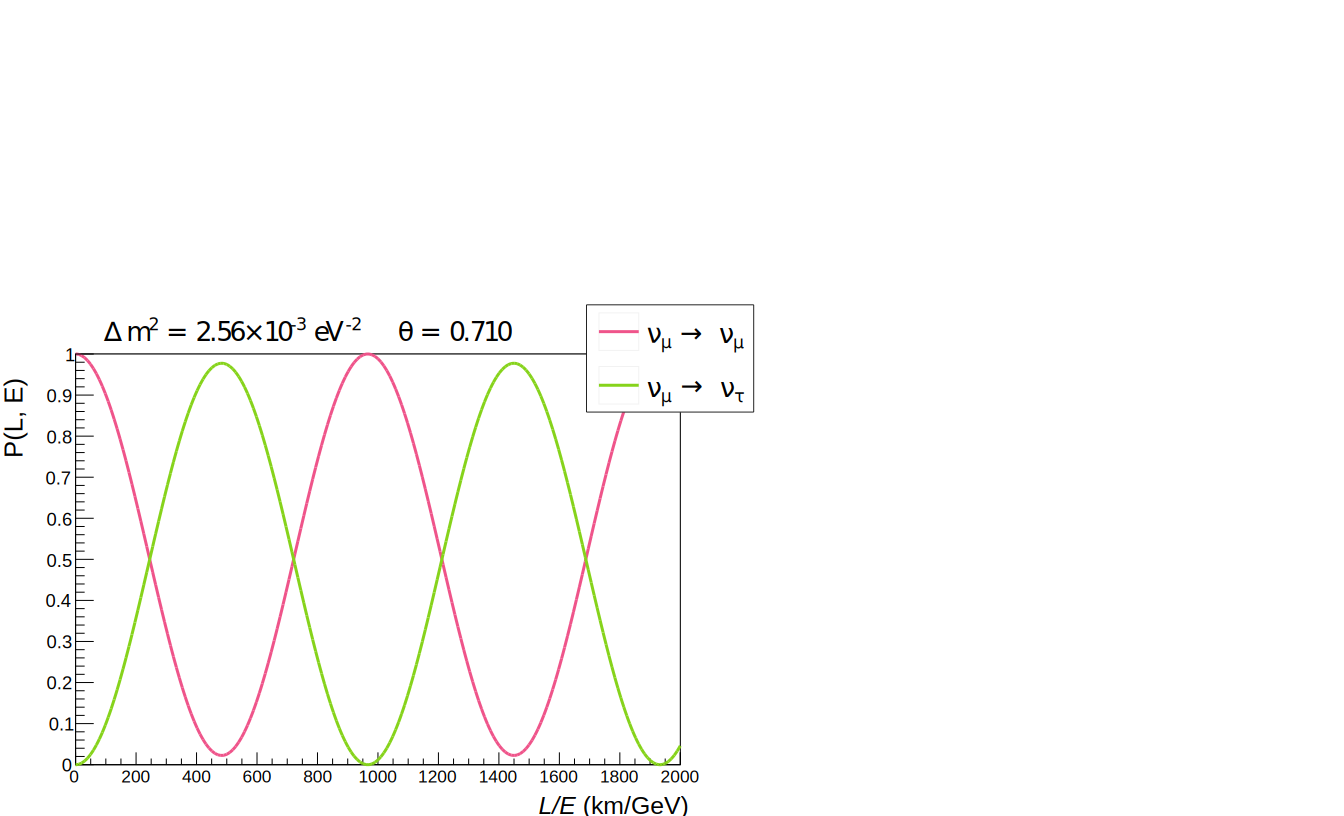
\includegraphics[width=0.6\textwidth]{twonu.pdf}
	\captionsetup{width=0.9\textwidth}
	\caption{Oscillation probability vs. $L/E$ for two neutrino flavours. The
	amplitude is governed by $\theta$ while the frequency is proportional to
	$\Delta m^2$. The mixing between flavours is almost maximal, i.e. the
	appearance of $\nu_\tau$ is almost 100\% at the half period.}
	\label{fig:twonu_plots}
\end{figure}
For this plot, we picked the parameters $\Delta m^2$ and $\theta$ (shown in
figure) from global fits of past experiments, reported by the Particle Data
Group (PDG)\cite{pdg}.

\begin{wraptable}{r}[2cm]{0.36\textwidth}
	\captionsetup{justification=centering}
	\centering
\begin{tabular}{ | c | c | }
	\hline
	Parameter & Value\\\hline
	$\Delta m^2_{21}$ & \SI{7.37e-5}{\eV^{-2}}\\
	$|\Delta m^2_{31}|$ & \SI{2.56e-3}{\eV^{-2}}\\
	$\theta_{12}$		  & 0.576\\
	$\theta_{23}$			& 0.710\\
	$\theta_{13}$ 		& 0.147\\\hline
\end{tabular}
	\caption{Parameter values used in fig.~\ref{fig:threenu_plots} and
	fig.~\ref{fig:dune_prob}}
	\label{tab:threenu_params}
\end{wraptable}

The next step is to implement three-neutrino oscillations. This involves
implementing the complex PMNS matrix of eq.~\ref{eq:PMNS} and the more general
probability function of eq.~\ref{eq:nuprob}. 
\begin{figure}
	\centering
	\makebox[1\textwidth][c]{
		\centering
	\begin{subfigure}[b]{0.6\textwidth}
		\centering
		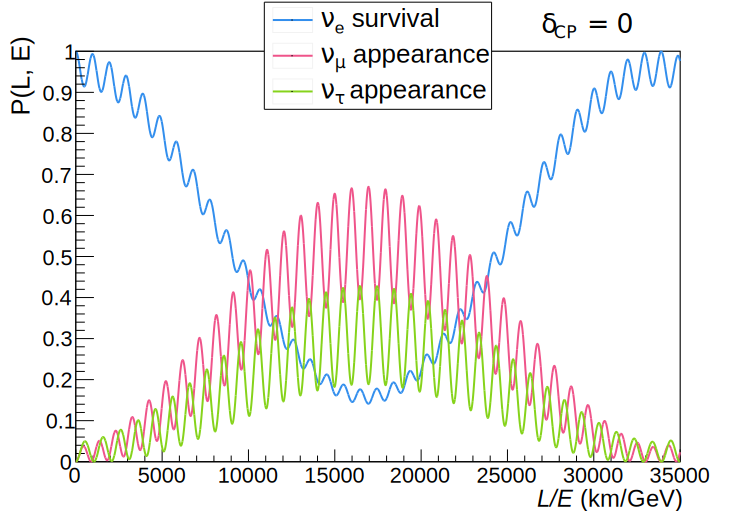
\includegraphics[width=\textwidth]{threenu_0.pdf}
	\end{subfigure}
	\begin{subfigure}[b]{0.6\textwidth}
		\centering
		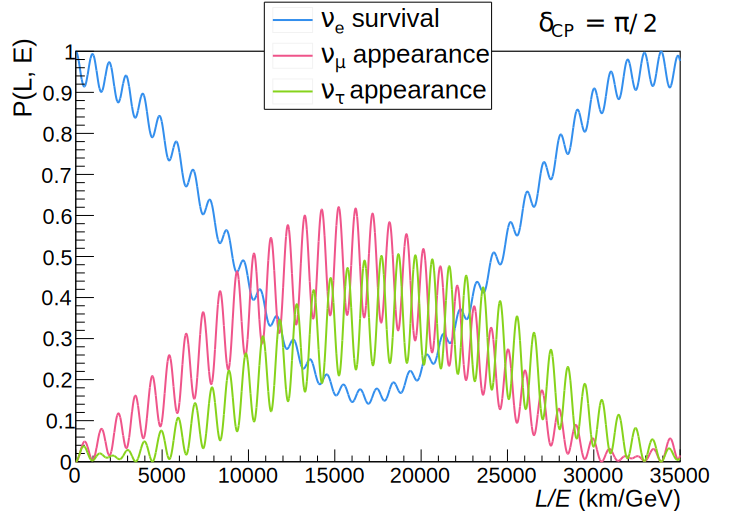
\includegraphics[width=\textwidth]{threenu_pihalf.pdf}
	\end{subfigure}}
\caption{Oscillation probability for a neutrino produced as a $\nu_e$, allowed to
	oscillate to $\nu_\tau$ and $\nu_\mu$. The mass hierarchy is NH for both
	plots. We illustrate the difference made by
	the CP-violating phase by showing a plot where CP is conserved
	($\delta_{CP}=0$) and a plot where CP is maximally violated ($\delta_{CP} =
	\pi/2$).}
\label{fig:threenu_plots}
\end{figure}
Figure~\ref{fig:threenu_plots} shows the oscillation probability for a neutrino
starting as a $\nu_e$ as a function of $L/E$. All parameters except
$\delta_{CP}$ are best-fit values listed by the PDG\cite{pdg} under the
assumption that the true mass hierarchy is normally ordered.
Table~\ref{tab:threenu_params} shows these values.


The difference between the two plots in figure~\ref{fig:threenu_plots} clearly
shows that given all other parameters, it is possible to determine the true
value of $\delta_{CP}$ by measuring neutrino appearance rates. Unfortunately,
the problem is not that easily solved. In neutrino experiments, reconstructing
the energy of neutrinos in the detector is difficult and prone to random and
systematic errors. Additionally, while some parameters are known with good
precision ($\theta_{12}, \theta_{13}, \Delta m^2_{21}$), the others remain
elusive and challenging to measure independently of each other.
Corrections must also be applied when the oscillations take place
through matter. It is necessary to choose an appropriate and reliable model of the
of the medium through which the neutrinos propagate, since the potential $V_e$ of
equation~\ref{eq:matter_potential} is proportional to the electron density in
the medium.


\section{Modelling an accelerator-based long baseline experiment}

\subsection{The DUNE experiment}
The Deep Underground Neutrino Experiment (DUNE) is a future long-baseline
experiment designed to --- among other goals --- determine the CP violating phase
$\delta_{CP}$, the neutrino mass hierarchy (the sign of $\Delta m^2_{31}$) and
the octant of $\theta_{23}$ (whether it is greater or less than 
$\pi/4$)\cite{cdr}. 
It will make use of Fermilab's Long-Baseline Neutrino Facility (LBNF) in Batavia,
Illinois for the production of a high-intensity neutrino beam aimed at the
Sanford Underground Research Facility, \SI{1300}{\km} away, where the DUNE
detectors will be built.
Four liquid argon time-projection chambers (LArTPC) of fiducial mass
\SI{10}{\kt} each will serve as detectors, with the ability to reconstruct the
trajectories and kinematic quantities of interacting neutrinos.
DUNE will primarily observe the oscillations from $\nu_\mu$ to $\nu_e$ in the
LBNF beam. This appearance channel alone is expected to provide enough data to
reach the objectives mentioned above, as we will show later.
The neutrino beam will travel through the Earth's crust for \SI{1300}{\km},
hence matter effects must be taken into account.

The DUNE experiment is thus a perfect candidate to try our simple model and see if
we can reproduce results from the literature, namely predictions on the
potential outcomes of the experiment.

\subsection{Event rate at the detector}
In order to predict an event rate $N$ in a general detector, we usually need three
elements: the luminosity of the beam $L$, the interaction cross section $\sigma$, and the
efficiency of the detector $\eps$:
\begin{equation}N = \eps L \sigma,\label{eq:rate}\end{equation}
where $L$ has units \si{\m^{-2} \s^{-1}}, $\sigma$ has units \si{\m^2} and
$\eps$ is unitless.
We will use a modified version of this approach to predict event rates inside
DUNE's liquid argon time-projection chamber (LArTPC), as a function of
energy. While our model
accurately describes the flavour oscillations of neutrinos, we are unable to
estimate the neutrino flux coming out of the LBNF accelerator, or the
efficiency of the LArTPC. For these two aspects we will rely on results
presented by the DUNE collaboration in their conceptual design report (CDR).

To produce the neutrinos, the LBNF accelerates protons which collide with a
graphite target to produce secondary mesons ($\pi^+, \pi^-$). These particles are focused
along a decay pipe where they decay into muons and their associated muon
neutrinos\cite{papadimitriou}. Hence by modelling the proton/target collision and the
decay of secondary mesons, one can estimate the flux of neutrinos produced by
the accelerator. The volume 3 of the CDR\cite{cdr_vol3} provides the predicted
flux of $\nu_\mu$ and $\nu_e$ at the detector in the absence of oscillations.
To produce these results, they use the \textsc{Geant4}\cite{Geant4} software to simulate
the beamline from the reference design of the LBNF accelerator.
Figure~\ref{fig:nuflux} shows a reproduction of the resulting plot from the DUNE CDR.
\begin{figure}
	\centering
	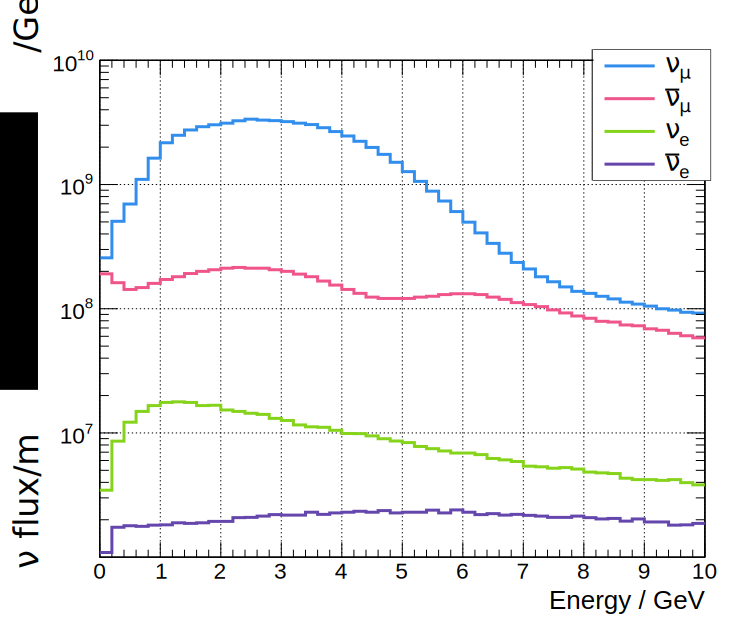
\includegraphics[width=0.5\textwidth]{dune_flux.pdf}
	\caption{Predicted neutrino flux at the DUNE detector in the absence of
	oscillations, when focusing positively charged pions through the decay pipe. 
	``POT'' stands for protons on target.
	Reproduction of figure 6-2 from the DUNE CDR Vol.
	3\cite{cdr_vol3}.}
	\label{fig:nuflux}
\end{figure}

It is fairly simple to convert this ``un-oscillated'' spectrum into an
``oscillated'' one. Typically in accelerator-based experiments, the observed oscillation channel
is the $\nu_\mu \rightarrow \nu_e$ appearance. Hence for each bin in the
spectrum of figure~\ref{fig:nuflux}, we multiply the un-oscillated
muon-neutrino flux
$\Phi^{(\mu)}_0$ (blue line) by the $\nu_\mu \rightarrow \nu_e$ oscillation
probability:
\begin{equation}
	\Phi^{(e)}_\text{osc} (E_i) = P_{\nu_\mu \rightarrow \nu_e} (E_i) \times
\Phi^{(\mu)}_0 (E_i),\label{eq:flux}\end{equation}
where $\Phi^{(e)}_\text{osc}$ is the flux of electron-neutrinos resulting from
$\nu_\mu$ oscillations, and $i$ indexes energy bins.
We show this $P_{\nu_\mu \rightarrow \nu_e}$ function for different values of
$\delta_{CP}$ and the two possible mass hierarchies on
figure~\ref{fig:dune_prob}. We also illustrate the influence of matter effects
on the appearance probability by showing oscillations in vacuum and in the
Earth's mantle.
\begin{figure}
	\centering
	\makebox[\textwidth][c]{
		\begin{subfigure}{0.6\textwidth}
		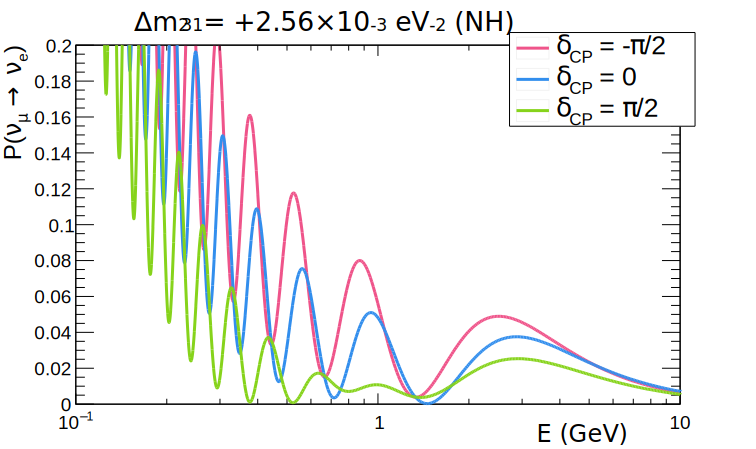
\includegraphics[width=\textwidth]{dune_prob_nh_vac.pdf}
			\caption{Vacuum, NH}\label{fig:vacNH}
		\end{subfigure}
		\begin{subfigure}{0.6\textwidth}
		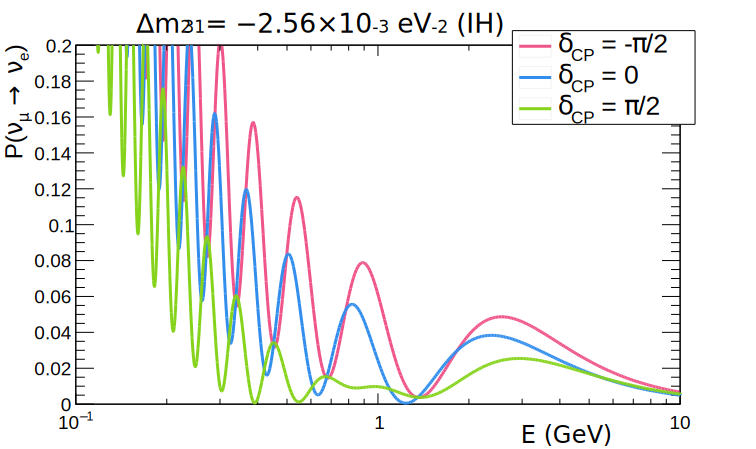
\includegraphics[width=\textwidth]{dune_prob_ih_vac.pdf}
			\caption{Vacuum, IH}\label{fig:vacIH}
		\end{subfigure}}
	\makebox[\textwidth][c]{
	\begin{subfigure}{0.6\textwidth}
		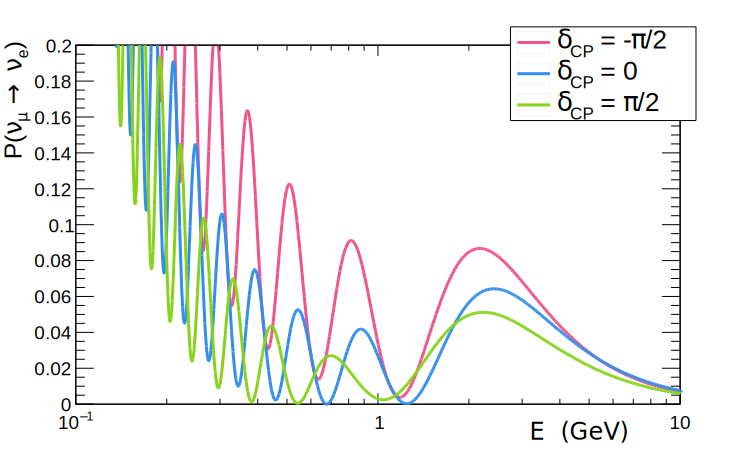
\includegraphics[width=\textwidth]{dune_prob_nh.pdf}
		\caption{Matter, NH}\label{fig:matNH}
		\end{subfigure}
		\begin{subfigure}{0.6\textwidth}
		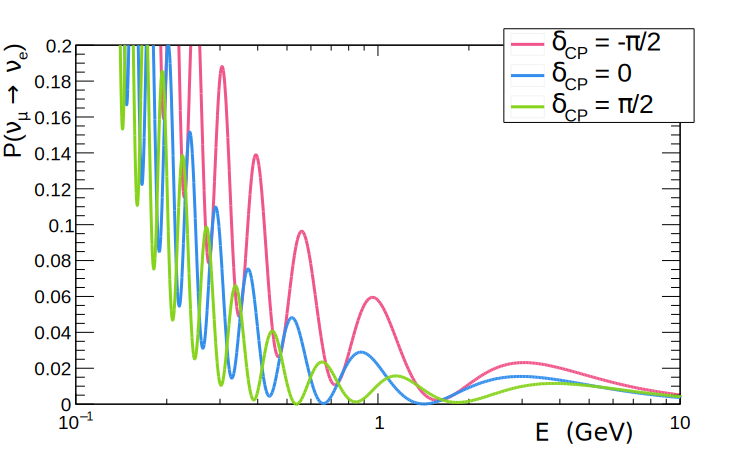
\includegraphics[width=\textwidth]{dune_prob_ih.pdf}
			\caption{Matter, IH}\label{fig:matIH}
		\end{subfigure}}
	\caption{Oscillation probability $\nu_\mu \rightarrow \nu_e$ as a function of
	neutrino energy for neutrinos travelling over a baseline $L=\SI{1300}{\km}$.
	Plots on the left have a normally ordered mass hierarchy, and plots on the
	right an inverted mass hierarchy. On top, neutrinos are oscillated in empty
	space, and on the bottom they are oscillated through matter of constant
	density $N_e=2.2 N_A~\si{\cm^{-3}}$, where $N_A$ is Avogadro's
	constant((citation needed)). All vacuum oscillation parameters are
	listed in table~\ref{tab:threenu_params}.}
\label{fig:dune_prob}
\end{figure}

In general, the first (rightmost) peak\footnote{It is the ``first peak''
because the probability falls to zero at higher energies. Note that the curves
in figure~\ref{fig:threenu_plots} had $L/E$ on the x-axis, while those in
figure~\ref{fig:dune_prob} are plotted against $E$. Hence the region covered by
the latter corresponds to the leftmost part of the former.} in the oscillation
probability will provide the best signal, since it is wider than all other
peaks on the energy axis, and thus easier to resolve.
The first oscillation peak for the DUNE baseline $L=\SI{1300}{\km}$ occurs between 1 and
\SI{10}{\GeV}, and thus it is the
energy range of choice for the DUNE experiment\cite{cdr}. 

It is interesting to observe that matter effects enhance the amplitude of
oscillations for the NH, and reduce it for the IH. The mass hierarchy only
influences the sign of one of the mass-squared differences, thus in a vacuum it
only affects the frequency of oscillations, as is shown on
figures~\ref{fig:vacNH} and~\ref{fig:vacIH}: the peak amplitudes are left
unchanged under a change of hierarchy. In vacuum, we can only change the
amplitude by changing the mixing angles. We see on figures~\ref{fig:matNH}
and~\ref{fig:matIH} that matter effects mix the parameters --- as is manifest
already for two neutrinos in equation~\ref{eq:deltam2m} --- in such a way that the
mass hierarchy can impact the amplitude as well. This feature is crucial to
DUNE's sensitivity to the mass hierarchy, as it will make discriminating
between the two hypotheses much easier than if the neutrinos were propagating
in empty space.

Now that we have the neutrino flux in the detector, i.e.~the luminosity
variable of equation~\ref{eq:rate}, we would normally need a model of the weak
interactions with the liquid argon ($\sigma$) and of the detector efficiency
($\eps$).
However another option is to normalize the flux to the integrated event rate,
i.e.~the total number of events expected to be observed during a given exposure
time. If we denote by $N_\text{int}$ this integrated event rate, then the
predicted event rate per unit energy is
\begin{equation}
	\frac{\md N}{\md E} = \frac{N_\text{int}}{\int \Phi^{(e)}_\text{osc} (E)~\md E}
	\times \Phi^{(e)}_\text{osc} (E).
\end{equation}
In other words, we first normalize the flux spectrum $\Phi^{(e)}_\text{osc}$ to
1 by dividing it by its integral, and then normalize to the integrated event
rate by multiplying by $N_\text{int}$.
Since our flux is a function of discrete energy bins, we can rewrite this as
\begin{align}
	\frac{N_i}{\Delta E} &= \frac{N_\text{int}}{\sum\limits_j \Phi^{(e)}_\text{osc} (E_j)
	\Delta E} \times \Phi^{(e)}_\text{osc} (E_i)\nonumber\\\implies
	N_i &= \frac{N_\text{int}}{\sum\limits_j \Phi^{(e)}_\text{osc} (E_j)} \times
	\Phi^{(e)}_\text{osc} (E_i),\label{eq:event_rate_0}
\end{align}
where $N_i$ is now the event rate per energy bin.
Thus, from the integrated event rate, we are able to retrieve the event rate as
a function of energy. We can then use this data to obtain the experiment's
sensitivity to the mass hierarchy and $\delta_{CP}$.

The CDR uses the \textsc{Genie}\cite{GENIE} neutrino event generator and a
parametrized detector response, to process the neutrino flux and
obtain an event rate through Monte Carlo simulations. This complex modelling
allows them to ``classify the types of neutrino interactions, including
backgrounds and misidentified interactions''\cite{LBNE}. 
Hence they are able to predict that the total number
of CC events from $\nu_e$ appearance between 0.5 and \SI{8}{\GeV} during an exposure of 150
kt$\cdot$MW$\cdot$year will be $N^\text{N}_\text{int}=861$ if the true hierarchy is normal,
and $N^\text{I}_\text{int}=495$ if it is inverted. Although both results assume that
$\delta_{CP}=0$, we will be able to calculate the event rates for all values of
$\delta_{CP}$ using our model.

As can be seen on any of the graphs of figure~\ref{fig:dune_prob}, the area under the first
appearance peak is different for different values of $\delta_{CP}$. This
indicates that the integrated event rate depends on $\delta_{CP}$.
The integrated event rate for any $\delta_{CP}$ is given by
\begin{align}
	N_\text{int} (\delta) &= \frac{\int P (
	\delta)~\md E}{\int P (
	\delta=0)~\md E} \times N_\text{int}\nonumber\\
		&= \frac{\sum_j \Phi_j (\delta) }{\sum\limits_j \Phi_j (\delta=0)} \times
	N_\text{int},\quad\text{using eq.~\ref{eq:flux},}\label{eq:int_event_rate}
\end{align}
where $P(\delta)$ is the $\nu_\mu\rightarrow\nu_e$ appearance probability
for any $\delta_{CP}=\delta$, and $\Phi_j \equiv \Phi^{(e)}_\text{osc}(E_j)$.
Thus, substituting into equation~\ref{eq:event_rate_0},
\begin{align}
	N_i (\delta) &= \frac{N_\text{int}(\delta)}{\sum\limits_j \Phi_j (\delta)}
	\times \Phi_i (\delta)\nonumber\\
	&= \frac{N_\text{int}}{\sum\limits_j \Phi_j (\delta)} \frac{\sum_j \Phi_j
	(\delta)}{\sum\limits_j \Phi_j (\delta=0)} \times \Phi_j(\delta)\nonumber\\
	&= \frac{N_\text{int}}{\sum\limits_j \Phi_j (\delta=0)} \times
	\Phi_j(\delta).\label{eq:event_rate}
\end{align}
Equation~\ref{eq:event_rate} allows us to calculate an event rate spectrum
for any $\delta_{CP}$ using the integrated event rate from the CDR and two
predicted fluxes we calculate using eq.~\ref{eq:flux}.
Figure~\ref{fig:event_rate} shows examples of such spectra, for two values of
$\delta_{CP}$ and the two possible hierarchies.
\begin{figure}
	\centering
	\makebox[\textwidth][c]{
	\begin{subfigure}{0.6\textwidth}
	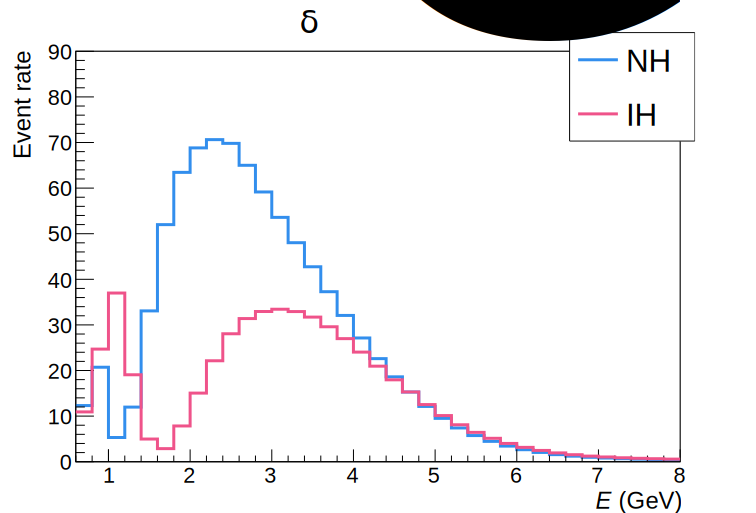
\includegraphics[width=\textwidth]{event_rate_0.pdf}
	\end{subfigure}
	\begin{subfigure}{0.6\textwidth}
		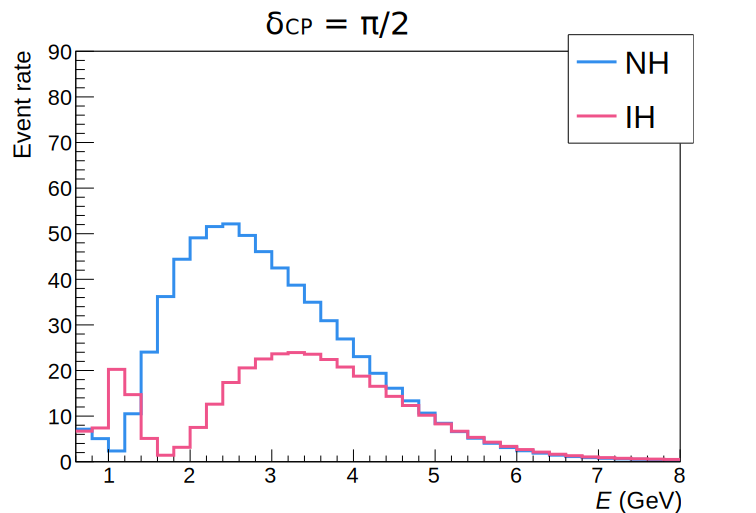
\includegraphics[width=\textwidth]{event_rate_pi.pdf}
	\end{subfigure}
	}
	\caption{Predicted event rate spectra at DUNE as a function of neutrino energy, for
	two values of $\delta_{CP}$ and the two hierarchies. For $\delta_{CP}=0$, the
	area under the curve (integrated event rate) is $N^\text{N}_\text{int}=861$ for the
	blue line and
	$N^\text{I}_\text{int}=495$ for the red line. For
	$\delta_{CP}=\pi/2$, the integrals are given by eq.~\ref{eq:int_event_rate}.}
\label{fig:event_rate}
\end{figure}

\subsection{Energy reconstruction}
In order to produce a more realistic model, we can introduce by hand
uncertainties on the energy reconstruction of neutrino events in the detector.
The method is very straightforward: for each event in each energy bin $i$, we
pick the reconstructed energy from a normal distribution around the true energy
$E_i$. The event is then reassigned to the bin corresponding to the
reconstructed energy.
\begin{figure}
	\centering
	\makebox[\textwidth][c]{
	\begin{subfigure}{0.6\textwidth}
	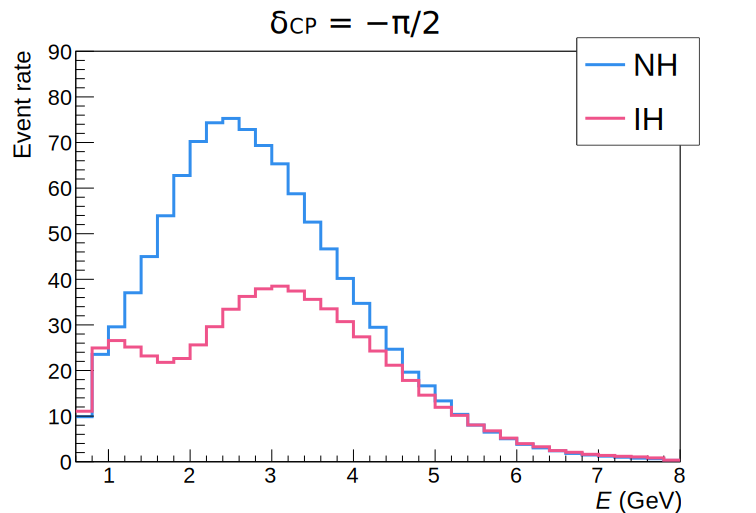
\includegraphics[width=\textwidth]{reconstructed_-.pdf}
	\end{subfigure}
	\begin{subfigure}{0.6\textwidth}
		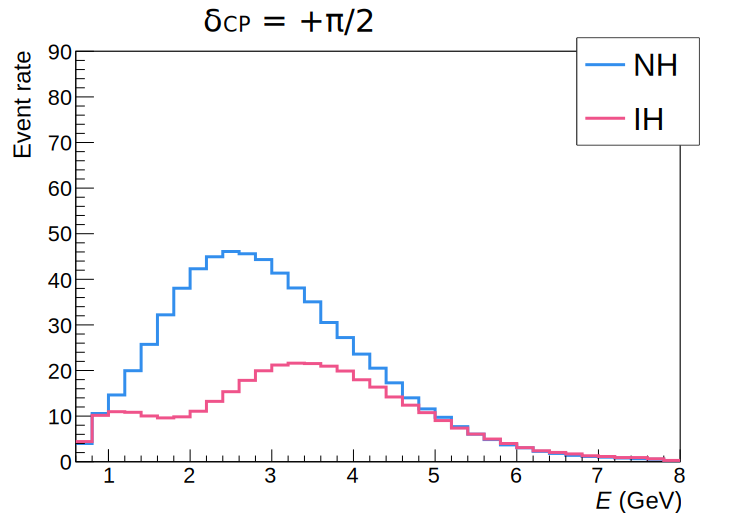
\includegraphics[width=\textwidth]{reconstructed_+.pdf}
	\end{subfigure}
	}
	\caption{Predicted event rate spectra at DUNE after energy reconstruction.
	The statistical uncertainty on the energy of each event is picked to be
	$\sigma_E = \SI{0.5}{\GeV}$.}
\label{fig:event_rate_reconstructed}
\end{figure}

Figure~\ref{fig:event_rate_reconstructed} shows examples of reconstructed event
rate spectra for $\delta_{CP}=-\pi/2$ and $\delta_{CP}=\pi/2$. We observe that
this simplistic energy reconstruction flattens out the event distribution, but
also slightly shifts the oscillation maxima towards the high energies, hence
introducing a systematic error in the event rate.

\subsection{Sensitivity to the mass hierarchy and CP violation}
With our event rate spectra under NH, IH, and any $\delta_{CP}$, we can finally
estimate the sensitivity of DUNE using the methods of
section~\ref{sec:statistics}. 
\begin{figure}
	\centering
	\makebox[\textwidth][c]{
\begin{subfigure}[b]{0.6\textwidth}
	\centering
	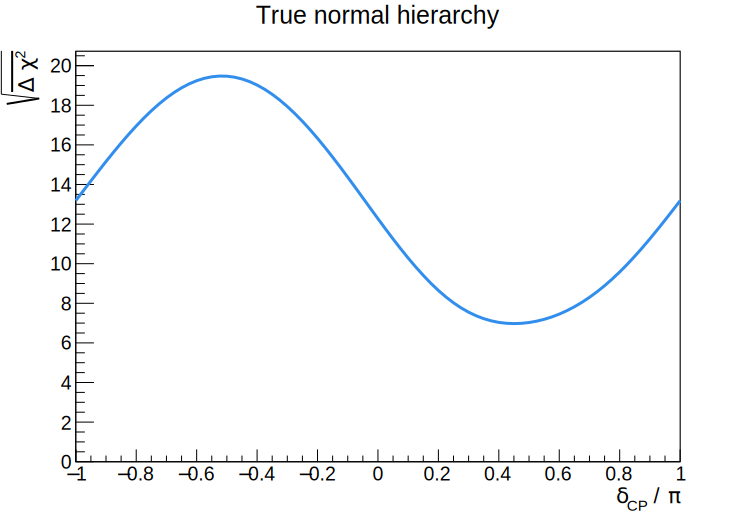
\includegraphics[width=\textwidth]{sens_mh_nh.pdf}
\end{subfigure}
\begin{subfigure}[b]{0.6\textwidth}
	\centering
	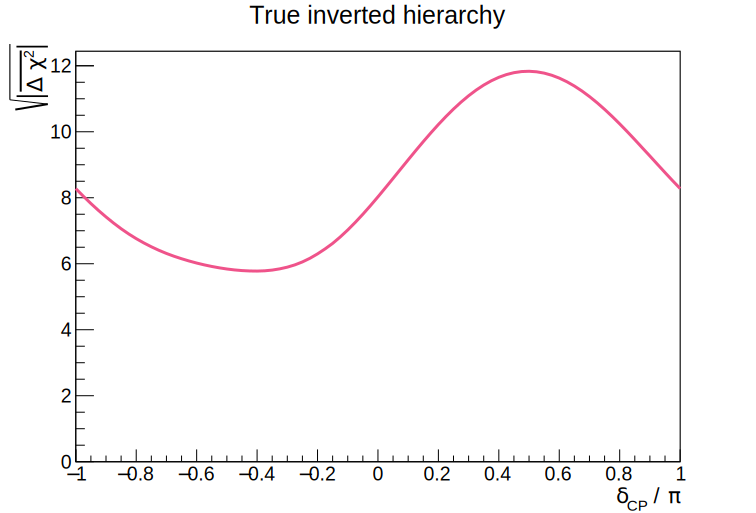
\includegraphics[width=\textwidth]{sens_mh_ih.pdf}
\end{subfigure}}
\caption{Minimum sensitivity of DUNE to the neutrino mass hierarchy as a
	function of $\delta_{CP}$ and the true hierarchy, for an exposure of
	150 kt$\cdot$MW$\cdot$year.}
	\label{fig:sens_mh}
\end{figure}

Figure~\ref{fig:sens_mh} shows the mass hierarchy sensitivity of DUNE as
defined in equation~\ref{eq:mean_dc2_mh_d}. 
Qualitatively, we can see that if
the mass hierarchy is normally ordered, DUNE will more efficiently determine it
if $\delta_{CP}$ lies around $-\pi/2$. On the other hand, if it is inverted, a $\delta_{CP}$
around $\pi/2$ will be more favourable. Under an inverted hierarchy, the
average sensitivity is lower than for NH, which can be explained by the overall smaller
number of events expected to be observed under IH. However,
$\overline{\Delta\chi^2}$ for the mass hierarchy is greater than 5 for all
values of $\delta_{CP}$ and both possible hierarchies, indicating that the
predicted potential for DUNE to determine the true mass hierarchy is
overwhelmingly good.
\begin{figure}
	\centering
	\makebox[\textwidth][c]{
\begin{subfigure}[b]{0.6\textwidth}
	\centering
	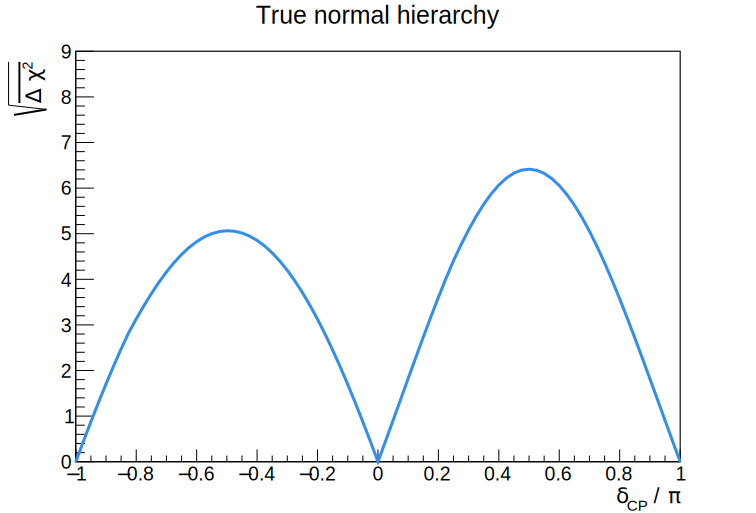
\includegraphics[width=\textwidth]{sens_cp_nh.pdf}
\end{subfigure}
\begin{subfigure}[b]{0.6\textwidth}
	\centering
	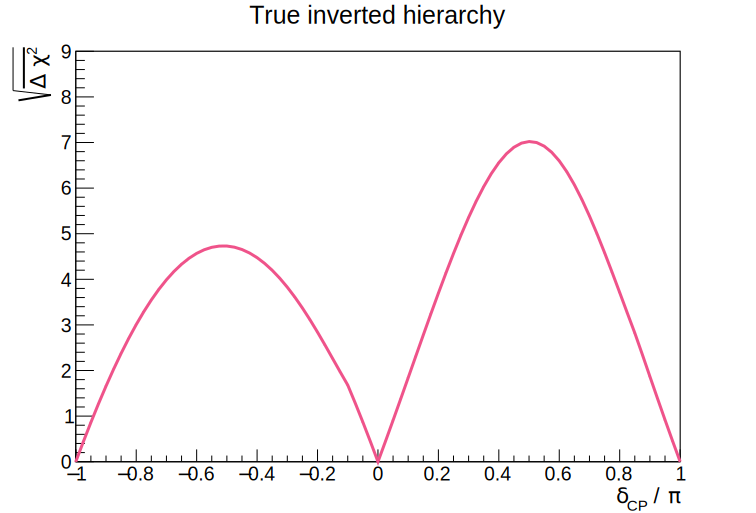
\includegraphics[width=\textwidth]{sens_cp_ih.pdf}
\end{subfigure}}
\caption{Sensitivity of DUNE to CP violation through neutrino oscillations, for an
	exposure of 150 kt$\cdot$MW$\cdot$year.}
\label{fig:sens_cp}
\end{figure}

Figure~\ref{fig:sens_cp} shows the sensitivity of DUNE to CP violation, as
defined in eq.~\ref{eq:dc2_cpv}.







%\chapter{Chapter 2 to N....}
%All reports will have at least one other chapter. These chapters are to explain what you did, your results, and your interpretation of those results. 

Discuss a draft outline with your supervisor. Review the mark scheme to make sure your chapters are addressing all the points mentioned.

\todo{You/your supervisor can use this method to add notes and suggestions}

\section{Section Title}
\label{sec:nameofsection}

\subsection{Subsections}

You should use subsections throughout your report. The more you divide up the text into standalone chunks, the easier it is to read.

\subsubsection{Subsubsections}

Subsubsections will be numbered in the text, but won't appear by default in the table of contents, unless to fiddle with the latex settings (probably not something you'd want to do if you are a beginner).

\paragraph{Headed Paragraphs} You can define paragraphs that start with bold headers, but these won't appear in the table of contents. 


\section{Referencing sections, tables, figures, equations}
Use the label command to make cross referencing a breeze. For example, this is how you would reference the Section above (see Section~\ref{sec:nameofsection}). This is how you would reference your conclusions chapter (see Chapter~\ref{ch:conclusions}).

\section{Referencing books, journal articles, webpages}

Here is an example of a book that has been included in the Bibliography \cite{MULLER2017}.

You will add the information required for the citation and the bibliography to the ref.bib file. The format of that file is very peculiar. Do not try to replicate it yourself. Instead, cut and paste the entries from an online archive (ask your supervisor for advice about this).

\section{Including Figures}

Here is an example of how you include a figure. Note that LaTeX will decide where to place the figure on the page. You can override that, but ask someone to help if you are a LaTeX novice.

\begin{figure}
 	\includegraphics[width=\linewidth]{images/ExampleFigure.pdf}
	\caption{Add a caption to all your figures. If the figure is not one you have made yourself, it is essential that you reference the source.}
	\label{fig:footprint}
\end{figure}


\section{Including Tables}

Here is an example of how you include a table. Note that LaTeX will decide where to place the table on the page. You can override that, but ask someone to help if you are a LaTeX novice.

\begin{table}
	\setlength{\tabcolsep}{.4em}
	\caption{Flat priors are specified with limits in square brackets, Gaussian priors with means $\pm$ standard deviations.}
	\begin{tabular}{lll}
		Parameter & Description & Prior \\ \hline
		$\log_{10}M_{\rm 200m}$ & Halo mass & $[11.0,18.0]$ \\
        $c_{\rm 200m}$ & Concentration & $[0,20]$\\
        $\tau$ & Dimensionless miscentering offset & $0.17\pm0.04$\\
		$f_{\rm mis}$ & Miscentered fraction & $0.25\pm0.08$\\
		$A_{m}$&Shape \& bias & \autoref{eq:multiplicative_total_bias}\\
		$B_0^{\rm cl}$ & Boost magnitude & $[0,\infty]$\\
		$R_s^{\rm cl}$ & Boost factor scale radius & $[0,\infty]$ \\
	\end{tabular}
    \label{tab:modeling_parameters}
\end{table}

\section{Including Equations}

Here is an example of a paragraph with an equation.

This shift is quantified as being dependent on the scaled mis-centering offset in terms of $r_\lambda$. We model the probabilistic distribution of $y$ as a Gaussian distribution:
\begin{equation}
y\sim\mathcal{N}(\bar{y}(x), \sigma_y (x)),
\end{equation} 
with the mean and the dispersion, $\bar{y}( x)$ and $\sigma_{y} ( x)$, both depending on $x$. Specifically, $\bar{y}( x)$ is chosen as a Gaussian function between $y$ and $x$, $\bar{y}(x)=\mathrm{exp}(-x^2/\alpha^2)$ with $\alpha$ being a model parameter. $\sigma_y (x)$ is chosen as $\sigma_y (x)=a\times\mathrm{arctan}(bx)$ and $a$ and $b$ are model parameters.

% make as many chapter files as you  need

\chapter{Conclusion}
\label{ch:conclusions}
\label{ch:conclusion}
Mention how we didn't take the antineutrino mode into account, which
theoretically increases sensitivity, especially CPV (?).  

We could have evaluated sensitivity as a function of exposure to see evolution
of significance over time.

We could have done this for more future experiments, eg T2HKK and PINGU-icecube.

We could have digged deeper in the statistics and evaluated ourselves through
MC the distribution of $dc2$ for MH and CPV.


All reports should include a conclusions chapter. This can be short. This can collate conclusions of previous chapters (these can be direct copies, rather than reworded, but ask your supervisor to check that this is OK in your specific context).

Some conclusions chapters will include a section describing future work. 

Take the opportunity to reflect on your experience. If you were able to go back in time 9 months, what advice would you give yourself?


\chapter*{Acknowledgements}
\addcontentsline{toc}{chapter}{Acknowledgments}
I am grateful to my supervisor, Dr. Lisa Falk, for being always insightful and
supportive.
I also thank my family for their backing and my friends for their inexhaustible
cynicism.

%doesn't need to be long. You can reference the preface, "e.g. my thanks to everyone that contributed to this project, see Preface."

%\chapter*{Bibliography}
%\addcontentsline{toc}{chapter}{Bibliography}
%\printbibliography

\begin{thebibliography}{100}


	\bibitem{cdr} DUNE Collaboration. Long-Baseline Neutrino Facility (LBNF) and
		Deep Underground Neutrino Experiment (DUNE) Conceptual Design Report Volume
		2: The Physics Program for DUNE at LBNF. \textit{Fermilab}.
		\href{https://arxiv.org/abs/1512.06148}{\texttt{arXiv:1512.06148}}. 2015.

	\bibitem{ROOT} The ROOT team. ROOT framework for data processing.
		\url{https://root.cern.ch}.

	\bibitem{hyperk} Hyper-Kamiokande proto-collaboration. Hyper-Kamiokande
		Design Report. \href{http://www.hyperk.org/?p=215}{\textit{KEK Preprint.}}
		2016.

	\bibitem{cdr-all} 
	DUNE Collaboration. Long-Baseline Neutrino Facility (LBNF) and
		Deep Underground Neutrino Experiment (DUNE) Conceptual Design Report.
		\href{https://web.fnal.gov/project/LBNF/ReviewsAndAssessments/LBNF_DUNE\%20DOE\%20CD-1\%20Refresh\%20Review/SitePages/Conceptual\%20Design\%20Report.aspx}{\textit{Fermilab}}.



	\bibitem{pauli} Pauli W.
		\href{http://microboone-docdb.fnal.gov/cgi-bin/RetrieveFile?docid=953;filename=pauli\%20letter1930.pdf}{Open letter to the group of radioactive people at the 
Gauverein meeting in Tübingen}. 4 Dec 1930.
	\bibitem{cowan} Cowan C L Jr, Reines F, Harrison F B, Kruse H W, McGuire A D.
		Detection of the Free Neutrino: a Confirmation. \textit{Science,
		\textbf{124}, 3212.} 1956.
	%\bibitem{fermi} Fermi E. Versuch einer Theorie der $\beta$-Strahlen. I.
	%	\textit{Z. Physik}. 1934.
	\bibitem{zuber} Zuber K. Neutrino
		Oscillations. \textit{IOP Publishing}. 2004.
	\bibitem{pontecorvo} Pontecorvo B. Electron and muon neutrinos.
		\textit{Soviet Physics JETP, \bf{10}, 1236}. 1960. Reprinted in
		Cambridge Monographs on Particle Physics, Nuclear Physics, and Cosmology,
		edited by Winter K. \textit{Cambridge University Press}. 1991.
	\bibitem{danby} Danby G, Gaillard J-M, Goulianos K, Lederman L M, Mistry N,
		Schwartz M, Steinberger J. Observation of High-Energy Neutrino Reactions
		and the Existence of Two Kinds of Neutrinos. \textit{Phys. Rev. Letters,
		\bf{9}, 1}. 1962.
	\bibitem{pontecorvo-osc} Pontecorvo B. Neutrino experiments and the problem of
		conservation of leptonic charge. \textit{Soviet Physics JETP, \textbf{26},
		984.} 1968.
	\bibitem{donut} DONUT Collaboration. Observation of Tau Neutrino
		Interactions.
		\href{https://arxiv.org/abs/hep-ex/0012035}{\texttt{arXiv:hep-ex/0012035}}.
		2000.

	\bibitem{smirnov} Smirnov A Yu. Solar neutrinos: Oscillations or
		No-oscillations?
		\href{https://arxiv.org/abs/1609.02386}{\texttt{arXiv:1609.02386}}. 2016.



		

	\bibitem{schwichtenberg} Schwichtenberg J. Physics From Symmetry (2nd Ed.).
		\textit{Springer International Publishing.} 2018.

	\bibitem{superk} The Super-Kamiokande Collaboration. Evidence for oscillation
		of atmospheric neutrinos.
		\href{https://arxiv.org/abs/hep-ex/9807003}{\texttt{arXiv:hep-ex/9807003}}. 1998.

	\bibitem{cohen} Cohen A, Glashow S, Ligeti Z. Disentangling neutrino
		oscillations. \textit{Physics Letters B, \textbf{678}, Issue 2.} 2008.

	\bibitem{langacker} Langacker P. The Standard Model and Beyond (2nd Ed.).
		\textit{CRC Press}. 2017.

	\bibitem{wolfenstein} Wolfenstein L. Neutrino oscillations in matter.
		\textit{Phys. Rev. D \textbf{17}, 2369}. 1978.

	\bibitem{mikheyev-smirnov} Mikheyev S, Smirnov A. Resonance enhancement of
		oscillations in matter and solar neutrino spectroscopy. \textit{Soviet
		Journal of Nuclear Physics \textbf{42:6}.} 1985.

	\bibitem{ricciardi} Ricciardi S. Lecture Notes on Neutrino oscillations in
		matter.
		\url{http://hepwww.rl.ac.uk/ricciardi/Lectures/MSW-1.pdf}. 2013.

	\bibitem{ohlsson} Ohlsson T, Snellman H. Three flavor neutrino oscillations
		in matter.
		\href{https://arxiv.org/abs/hep-ph/9910546v4}{\texttt{arXiv:hep-ph/9910546}}. 1999.

	\bibitem{kneller} Kneller J, McLaughlin G. Three Flavor Neutrino Oscillations
		in Matter: Flavor Diagonal Potentials, the Adiabatic Basis and the CP
		phase. \href{https://arxiv.org/abs/0904.3823}{\texttt{arXiv:0904.3823}}. 2009.

	\bibitem{davis} Davis R Jr, Harmer D, Hoffman K. Search for Neutrinos from
		the Sun. \textit{Phys. Rev. Lett. \textbf{20}, 1205}. 1968.
	\bibitem{sno} SNO Collaboration. Measurement of the Rate of $\nu_e + d
		\rightarrow p + p + e^-$ 
		Interactions Produced by $^8B$ Solar Neutrinos at the Sudbury Neutrino
		Observatory. \textit{Phys. Rev. Lett. \textbf{87}, 071301}. 2001.
	\bibitem{superk-solar} Super-Kamiokande Collaboration. Solar $^8B$ and hep
		Neutrino Measurements from 1258 Days of Super-Kamiokande Data.
		\textit{Phys. Rev. Lett. \textbf{86}, 5651}. 2001.

	\bibitem{kamland} KamLAND Collaboration.  First Results from KamLAND:
		Evidence for Reactor Anti-Neutrino Disappearance. \textit{Phys. Rev. Lett.
		\textbf{90}, 021802}. 2003.

	\bibitem{minos} MINOS Collaboration. Combined Analysis of $\nu_\mu$
		Disappearance and $\nu_\mu\rightarrow \nu_e$ Appearance in MINOS Using
		Accelerator and Atmospheric Neutrinos. \textit{Phys. Rev. Lett.
		\textbf{112}, 191801}. 2014.

	\bibitem{nova} NO$\nu$A Collaboration. Measurement of the Neutrino Mixing
		Angle $\theta_{23}$ in NO$\nu$A. \textit{Phys. Rev. Lett. \textbf{118},
		151802}. 2017.

	\bibitem{t2k} T2K Collaboration. Combined Analysis of Neutrino and
		Antineutrino Oscillations at T2K. \textit{Phys. Rev. Lett.
		\textbf{118}, 151801}. 2017.

	\bibitem{t2k-13} T2K Collaboration. Indication of Electron Neutrino
		Appearance from an Accelerator-Produced Off-Axis Muon Neutrino Beam.
		\textit{Phys. Rev. Lett. \textbf{107}, 041801}. 2011.


	\bibitem{dayabay} Daya Bay Collaboration. Observation of
		Electron-Antineutrino Disappearance at Daya Bay. \textit{Phys. Rev. Lett.
		\textbf{108}, 171803}. 2012.
	\bibitem{reno} RENO Collaboration. Observation of Reactor Electron
		Antineutrinos Disappearance in the RENO Experiment. \textit{Phys. Rev. Lett. \textbf{108},
		191802}. 2012.
	\bibitem{chooz} Double Chooz Collaboration. Indication of Reactor
		$\overline{\nu}_e$ Disappearance in the Double Chooz Experiment.
		\textit{Phys. Rev. Lett. \textbf{108}, 131801}. 2012.

	%\bibitem{gonzalez-garcia} Gonzalez-Garcia M, Maltoni M, Pe$\tilde{\text{n}}$a-Garay C,
	%	Valle J. Global three–neutrino oscillation analysis of
	%	neutrino data.
	%	\href{https://arxiv.org/abs/hep-ph/0009350}{\texttt{arXiv:hep-ph/0009350}}.
	%	2000.

	\bibitem{pdg} Particle Data Group. Review of Neutrino Masses, Mixing and
		Oscillations.
		\url{https://http://pdg.lbl.gov/2017/reviews/rpp2017-rev-neutrino-mixing.pdf}.
		2017.

	%\bibitem{novat23} The NOvA Collaboration. Measurement of the neutrino mixing
	%	angle $\theta_{23}$ in NOvA.
	%	\href{https://arxiv.org/abs/1701.05891}{\texttt{arXiv:1701.05891}}. 2017.
	\bibitem{raut} Raut S. Synergies and complementarities between proposed
		future neutrino projects.
		\href{https://arxiv.org/abs/1712.02096v1}{\texttt{arXiv:1712.02096}}.
		2017.

	\bibitem{thomson} Thomson M. Modern Particle Physics. \textit{Cambridge
		University Press}. 2013.


	\bibitem{blennow} Blennow M, Coloma P, Huber P, Schwetz T. Quantifying the
		sensitivity of oscillation experiments to the neutrino mass hierarchy.
		\href{https://arxiv.org/pdf/1311.1822.pdf}{\texttt{arXiv:1311.1822}}. 2013.

	\bibitem{ciuffoli} Ciuffoli E, Evslin J, Zhang X. Sensitivity to the
		Neutrino Mass Hierarchy.
		\href{https://arxiv.org/abs/1305.5150v4}{\texttt{arXiv:1305.5150}}. 2013.
	\bibitem{qian} Qian X, Tan A, Wang W, Ling JJ, McKeown RD, Zhang C.
		Statistical Evaluation of Experimental Determinations of Neutrino Mass
		Hierarchy.
		\href{https://arxiv.org/abs/1210.3651}{\texttt{arXiv:1210.3651}}. 2012.

	%\bibitem{barger} Barger V, Marfatia D, Whisnant K. Breaking Eight–fold
	%	Degeneracies in Neutrino CP Violation, Mixing, and Mass Hierarchy.
	%	\href{https://arxiv.org/abs/hep-ph/0112119}{\texttt{arXiv:hep-ph/0112119}}.
	%	2001.




	\bibitem{papadimitriou} Papadimitriou V, et al. Design of the LBNF beamline.
		\href{https://arxiv.org/abs/1704.04471}{\texttt{arXiv:1704.04471}}. 2017.

	\bibitem{cdr_vol3} DUNE Collaboration. Long-Baseline Neutrino Facility (LBNF)
		and Deep Underground Neutrino Experiment (DUNE) Conceptual Design Report
		Volume 3: Long-Baseline Neutrino Facility for DUNE. \textit{Fermilab}. 2015.





	\bibitem{Geant4} The \textsc{Geant4} Collaboration.
		\textsc{Geant4} --- a simulation toolkit. \textit{Nuclear Instruments and Methods in
		Physics Research, \textbf{506}, Issue 3.} 2003. 

	% Matter electron density source
	\bibitem{freund} Freund M, Ohlsson T. Matter Enhanced Neutrino Oscillations
		with a Realistic Earth Density Profile.
		\href{https://arxiv.org/abs/hep-ph/9909501}{\texttt{arXiv:hep-ph/9909501}}.
		1999.

	\bibitem{GENIE} Andreopoulos C, et al. The \textsc{GENIE} Neutrino Monte
		Carlo Generator.
		\href{https://arxiv.org/abs/0905.2517}{\texttt{arXiv:0905.2517}}. 2009.



	\bibitem{ballett} Ballett P, King S, Pascoli S, Prouse N, Wang T.
		Sensitivities and synergies of DUNE and T2HK. \href{
		https://arxiv.org/pdf/1612.07275.pdf}{\texttt{arXiv:1612.07275}}. 2016.
	\bibitem{martin-albo} Martin-Albo J. Sensitivity of DUNE to long-baseline
		neutrino oscillation physics.
		\href{https://arxiv.org/abs/1710.08964}{\texttt{arXiv:1710.08964}}. 2017.

	\bibitem{laguna-lbno} LAGUNA-LBNO Collaboration. The LBNO long-baseline
		oscillation sensitivities with two conventional neutrino beams at different
		baselines.
		\href{https://arxiv.org/abs/1412.0804}{\texttt{arXiv:1412.0804}}. 2014.

	\bibitem{masud} Masud M, Mehta P. Non-standard interactions spoiling the CP
		violation sensitivity at DUNE and other long baseline experiments.
		\href{https://arxiv.org/abs/1603.01380}{\texttt{arXiv:1603.01380}}. 2016.

	\bibitem{t2hkk} Hyper-Kamiokande proto-collaboration. Physics Potentials with
		the Second Hyper-Kamiokande Detector in Korea.
		\href{https://arxiv.org/abs/1611.06118}{\texttt{arXiv:1611.06118}}. 2016.
	%\bibitem{MNS} Maki Z, Nakagawa M, Sakata S. Remarks on the Unified Model of
	%	Elementary Particles. \textit{Progress of Theoretical Physics}. 1962.

	%\bibitem{pdg-ckm} Particle Data Group. Review of CP Violation in the Quark Sector.
	%	\url{http://pdg.lbl.gov/2017/reviews/rpp2017-rev-cp-violation.pdf}. 2017

	%\bibitem{LBNE} The LBNE Collaboration. The Long-Baseline Neutrino Experiment:
	%	Exploring Fundamental Symmetries of the Universe.
	%	\textit{Fermilab.}
	%	\href{https://arxiv.org/abs/1307.7335}{\texttt{arXiv:1307.7335}}. 2014.

\end{thebibliography}



\end{document}
